% Generálva: html/build_tex.js (o03.js). Kézzel ne szerkeszd, a forrás a html/data mappa.
\setcounter{chapter}{2}
\chapter{\texorpdfstring{Digitális alapsávi átvitel (PAM, ISI)}{Digitális alapsávi átvitel (PAM, ISI)}}\label{f3}
Elemi jelből szemábra, ISI és a többszintű rendszer próbája, valamint az emelt koszinuszos spektrum leolvasása.

\section{Alapok, egyszerűen}
\subsection{\texorpdfstring{A1. Jelölések és a minta képlete}{A1. Jelölések és a minta képlete}}\label{b3-jel}
\par\noindent{\small\renewcommand{\arraystretch}{1.25}\begin{tabularx}{\linewidth}{@{}>{\raggedright\arraybackslash}X>{\raggedright\arraybackslash}X@{}}\toprule
\textbf{Jel} & \textbf{Jelentés}\\\midrule
undefined & a undefined-adik szimbólum értéke (binárisnál undefined, négyszintűnél undefined)\\
undefined & elemi jel: egyetlen undefined szimbólum hatására a vevőben megjelenő jel\\
undefined & az elemi jel értéke a saját mintavételi pillanatában\\
undefined & az elemi jel értéke egy jelzési idővel később (ez lóg át a következő szimbólumba)\\
undefined & jelzési idő\\
undefined & az elemi jel spektruma\\
\bottomrule\end{tabularx}}\par

A PAM-jel az eltolt elemi jelek összege, $x(t)=\sum_kd_kh(t-kT)$. Ha a $k$-adik mintát a saját elemi jele $h_0$-nál, az előző szimbólumé $h_1$-nél metszi, akkor

\begin{center}\adjustbox{max width=\linewidth}{$\displaystyle x_k=h_0d_k+h_1d_{k-1}$}\end{center}

A második tag a \textbf{szimbólumközti áthallás (ISI)}. A döntés akkor hibátlan, ha a legrosszabb esetben is a jó oldalon marad a küszöbnek. $M$ szintnél a küszöbök a névleges szintek ($h_0d$) között félúton vannak.

\subsection{\texorpdfstring{A2. Nyquist-feltétel, emelt koszinusz}{A2. Nyquist-feltétel, emelt koszinusz}}\label{b3-nyq}
Az ISI akkor tűnik el, ha a spektrum $1/T$-nként eltolt másolatainak összege állandó. Az emelt koszinuszos spektrum ilyen: $f_1=(1-\alpha)/(2T)$-ig lapos, $f_2=(1+\alpha)/(2T)$-re nullára csökken, és a lecsengés a $1/(2T)$ pontra (ahol az érték a fele) pontszimmetrikus. Ebből $1/(2T)=(f_1+f_2)/2$ és $\alpha=(f_2-f_1)/(f_2+f_1)$.

% ------------------------------------------------------------------
\section{\texorpdfstring{3.1. feladat: Elemi jel 1,15 és 0,25}{3.1. feladat: Elemi jel 1,15 és 0,25}}\label{o3_01}
\setcounter{lepes}{0}
\begin{feladat}{3.1. feladat}
Bináris PAM, $h=1{,}15$ a $[0,T]$-n, $0{,}25$ a $[T,2T]$-n. a) PAM jel a \ldots{}0-1-1-0-0-1\ldots{} sorra. b) Van-e ISI, ha $t_0=3T/4$? c) Négyszintű szemábra ($-3,-1,+1,+3$), alkalmas-e?

{\footnotesize\sffamily Forrás: 5-ösöm 10. oldal $\cdot$ 5o\_10\_1. Címkék: vizsga}
\end{feladat}
\begin{keresunk}
\begin{itemize}
\item a) $x(t)$ (a PAM-jel) szintjei a bitsorra
\item b) van-e ISI, és okoz-e hibát
\item c) nyitott-e a négyszintű szem
\end{itemize}
\end{keresunk}
\begin{jeloles}
\begin{jeltabla}
$h$ & az elemi jel: 1,15 az első és 0,25 a második jelzési időben & \\
$T$ & jelzési idő & \\
$d_k$ & a k-adik szimbólum (+1 vagy $-$1) & \\
$\ca{t_0}$ & a mintavétel helye a jelzési időn belül & $3$\\
$x$ & a mintavevő kimenete (egy minta értéke) & \emph{keresett}\\
$k$ & az időrés sorszáma & \\
$x_k$ & a k-adik időrésben vett minta & \\
$d_{k-1}$ & az előző szimbólum (+1 vagy $-$1) & \\
$h_0$ & az elemi jel: 1,15 az első és 0,25 a második jelzési időben & \\
$h_1$ & az elemi jel: 1,15 az első és 0,25 a második jelzési időben & \\
$d$ & a szimbólum értéke, +1 az 1-es és $-$1 a 0-s bitre & \\
\end{jeltabla}
\end{jeloles}

\lepes{A minták képlete}
A $k$-adik időrésben ($kT$ és $(k+1)T$ között) a saját elemi jel első szakasza (1,15) és az előző szimbólum elemi jelének második szakasza (0,25) adódik össze. A $3T/4$-es mintavétel ebbe az időrésbe esik, így ez a minta is.

\begin{center}\adjustbox{max width=\linewidth}{$\displaystyle x_k=1{,}15\,d_k+0{,}25\,d_{k-1}$}\end{center}
\jegyzet{definíció}{$h_0=1{,}15$, $h_1=0{,}25$}

\lepes{a) A PAM-jel a bitsorra}
A bitsor $d=-1,+1,+1,-1,-1,+1$. Minden időrésre behelyettesítünk (az elsőhöz az előző bit nem ismert).

\begin{center}\adjustbox{max width=\linewidth}{$\displaystyle +1\text{ után }-1:\ 1{,}15-0{,}25=0{,}9\qquad+1\text{ után }+1:\ 1{,}15+0{,}25=1{,}4$}\end{center}
\jegyzet{behelyettesítés}{}

\begin{center}\adjustbox{max width=\linewidth}{$\displaystyle -1\text{ után }+1:\ -1{,}15+0{,}25=-0{,}9\qquad-1\text{ után }-1:\ -1{,}4$}\end{center}
\jegyzet{behelyettesítés}{}

\begin{center}\adjustbox{max width=\linewidth}{$\displaystyle x:\ -1{,}15\pm0{,}25,\ 0{,}9,\ 1{,}4,\ -0{,}9,\ -1{,}4,\ 0{,}9$}\end{center}
\jegyzet{számérték}{a hat időrés szintjei}

\lepes{b) ISI}
A minta értéke függ az előző bittől (0,9 vagy 1,4), tehát \textbf{van ISI}. Hibát viszont nem okoz: a döntési küszöb 0, és a legkisebb abszolút érték is $0{,}9>0$. A szem nyitott, a nyílása $2\cdot0{,}9=1{,}8$.

\lepes{c) Négyszintű rendszer}
Most $d_k\in\{-3,-1,1,3\}$, a névleges szintek $\pm1{,}15$ és $\pm3{,}45$, a küszöbök félúton: $0$ és $\pm2{,}3$. Az áthallás legfeljebb $0{,}25\cdot3=0{,}75$, mert $|d_{k-1}|\le3$.

\begin{center}\adjustbox{max width=\linewidth}{$\displaystyle d_k=1:\ 1{,}15-0{,}75=0{,}4>0\quad\text{és}\quad1{,}15+0{,}75=1{,}9<2{,}3$}\end{center}
\jegyzet{behelyettesítés}{a 0 és a 2,3 küszöb között marad}

\begin{center}\adjustbox{max width=\linewidth}{$\displaystyle d_k=3:\ 3{,}45-0{,}75=2{,}7>2{,}3$}\end{center}
\jegyzet{behelyettesítés}{a 2,3 felett marad}

\begin{center}\adjustbox{max width=\linewidth}{$\displaystyle 0{,}4>0$}\end{center}
\jegyzet{ellenőrzés}{a legrosszabb eset is a jó oldalon: alkalmas}

\begin{rajz}
\textbf{A PAM-jel a \ldots{}0-1-1-0-0-1\ldots{} bitsorra}\par
\begin{center}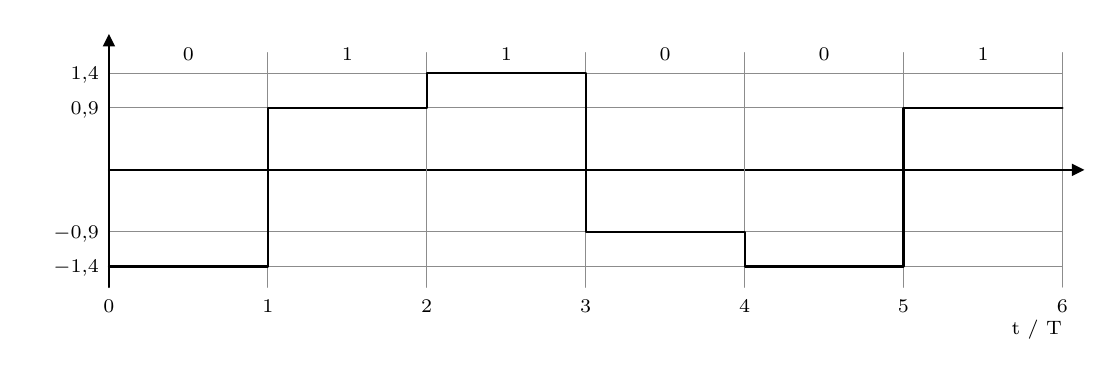
\begin{tikzpicture}[x=0.01985cm,y=-0.01985cm,line cap=round,line join=round]
\useasboundingbox (0,0) rectangle (680,200);
\path[draw=black!45,line width=0.35pt] (52,166) -- (52,16);
\path[draw=black!45,line width=0.35pt] (153.7,166) -- (153.7,16);
\path[draw=black!45,line width=0.35pt] (255.3,166) -- (255.3,16);
\path[draw=black!45,line width=0.35pt] (357,166) -- (357,16);
\path[draw=black!45,line width=0.35pt] (458.7,166) -- (458.7,16);
\path[draw=black!45,line width=0.35pt] (560.3,166) -- (560.3,16);
\path[draw=black!45,line width=0.35pt] (662,166) -- (662,16);
\path[draw=black!45,line width=0.35pt] (52,29.2) -- (662,29.2);
\path[draw=black!45,line width=0.35pt] (52,51.3) -- (662,51.3);
\path[draw=black!45,line width=0.35pt] (52,130.7) -- (662,130.7);
\path[draw=black!45,line width=0.35pt] (52,152.8) -- (662,152.8);
\path[draw=black,line width=0.7pt] (52,91) -- (670,91);
\path[fill=black,draw=none] (676,91) -- (668,87) -- (668,95) -- cycle;
\path[draw=black,line width=0.7pt] (52,166) -- (52,10);
\path[fill=black,draw=none] (52,4) -- (48,12) -- (56,12) -- cycle;
\node[anchor=base,inner sep=0pt,font=\scriptsize] at (52,182) {0};
\node[anchor=base,inner sep=0pt,font=\scriptsize] at (153.7,182) {1};
\node[anchor=base,inner sep=0pt,font=\scriptsize] at (255.3,182) {2};
\node[anchor=base,inner sep=0pt,font=\scriptsize] at (357,182) {3};
\node[anchor=base,inner sep=0pt,font=\scriptsize] at (458.7,182) {4};
\node[anchor=base,inner sep=0pt,font=\scriptsize] at (560.3,182) {5};
\node[anchor=base,inner sep=0pt,font=\scriptsize] at (662,182) {6};
\node[anchor=base east,inner sep=0pt,font=\scriptsize] at (46,33.2) {1,4};
\node[anchor=base east,inner sep=0pt,font=\scriptsize] at (46,55.3) {0,9};
\node[anchor=base east,inner sep=0pt,font=\scriptsize] at (46,134.7) {$-$0,9};
\node[anchor=base east,inner sep=0pt,font=\scriptsize] at (46,156.8) {$-$1,4};
\node[anchor=base east,inner sep=0pt,font=\scriptsize] at (662,196) {t / T};
\path[draw=black!45,line width=0.35pt,dash pattern=on 3pt off 2pt] (153.7,166) -- (153.7,16);
\path[draw=black!45,line width=0.35pt,dash pattern=on 3pt off 2pt] (255.3,166) -- (255.3,16);
\path[draw=black!45,line width=0.35pt,dash pattern=on 3pt off 2pt] (357,166) -- (357,16);
\path[draw=black!45,line width=0.35pt,dash pattern=on 3pt off 2pt] (458.7,166) -- (458.7,16);
\path[draw=black!45,line width=0.35pt,dash pattern=on 3pt off 2pt] (560.3,166) -- (560.3,16);
\path[draw=black,line width=0.8pt] (52,152.8) -- (153.7,152.8) -- (153.7,51.3) -- (255.3,51.3) -- (255.3,29.2) -- (357,29.2) -- (357,130.7) -- (458.7,130.7) -- (458.7,152.8) -- (560.3,152.8) -- (560.3,51.3) -- (662,51.3);
\node[anchor=base,inner sep=0pt,font=\scriptsize] at (102.8,21.3) {0};
\node[anchor=base,inner sep=0pt,font=\scriptsize] at (204.5,21.3) {1};
\node[anchor=base,inner sep=0pt,font=\scriptsize] at (306.2,21.3) {1};
\node[anchor=base,inner sep=0pt,font=\scriptsize] at (407.8,21.3) {0};
\node[anchor=base,inner sep=0pt,font=\scriptsize] at (509.5,21.3) {0};
\node[anchor=base,inner sep=0pt,font=\scriptsize] at (611.2,21.3) {1};
\end{tikzpicture}\end{center}
\begin{itemize}
\item Időrésenként egy vízszintes szakasz: $1{,}15\,d_k+0{,}25\,d_{k-1}$. Ha az előző bit ugyanaz, 1,4, ha más, 0,9 a szint (előjellel).
\item Az első időrésnél az előző bitet itt 0-nak ($-$1) vettük, ezért $-$1,4.
\end{itemize}

\textbf{Négyszintű szemábra a mintavételi pillanatban}\par
\begin{center}\begin{tikzpicture}[x=0.01985cm,y=-0.01985cm,line cap=round,line join=round]
\useasboundingbox (0,0) rectangle (680,230);
\path[draw=black!45,line width=0.35pt] (52,196) -- (52,16);
\path[draw=black!45,line width=0.35pt] (509.5,196) -- (509.5,16);
\path[draw=black!45,line width=0.35pt] (662,196) -- (662,16);
\path[draw=black!45,line width=0.35pt] (52,23.8) -- (662,23.8);
\path[draw=black!45,line width=0.35pt] (52,53.2) -- (662,53.2);
\path[draw=black!45,line width=0.35pt] (52,68.8) -- (662,68.8);
\path[draw=black!45,line width=0.35pt] (52,98.2) -- (662,98.2);
\path[draw=black!45,line width=0.35pt] (52,113.8) -- (662,113.8);
\path[draw=black!45,line width=0.35pt] (52,143.2) -- (662,143.2);
\path[draw=black!45,line width=0.35pt] (52,158.8) -- (662,158.8);
\path[draw=black!45,line width=0.35pt] (52,188.2) -- (662,188.2);
\path[draw=black,line width=0.7pt] (52,106) -- (670,106);
\path[fill=black,draw=none] (676,106) -- (668,102) -- (668,110) -- cycle;
\path[draw=black,line width=0.7pt] (52,196) -- (52,10);
\path[fill=black,draw=none] (52,4) -- (48,12) -- (56,12) -- cycle;
\node[anchor=base,inner sep=0pt,font=\scriptsize] at (52,212) {0};
\node[anchor=base,inner sep=0pt,font=\scriptsize] at (509.5,212) {3T/4};
\node[anchor=base,inner sep=0pt,font=\scriptsize] at (662,212) {T};
\node[anchor=base east,inner sep=0pt,font=\scriptsize] at (46,27.8) {4,2};
\node[anchor=base east,inner sep=0pt,font=\scriptsize] at (46,57.2) {2,7};
\node[anchor=base east,inner sep=0pt,font=\scriptsize] at (46,72.8) {1,9};
\node[anchor=base east,inner sep=0pt,font=\scriptsize] at (46,102.2) {0,4};
\node[anchor=base east,inner sep=0pt,font=\scriptsize] at (46,117.8) {$-$0,4};
\node[anchor=base east,inner sep=0pt,font=\scriptsize] at (46,147.2) {$-$1,9};
\node[anchor=base east,inner sep=0pt,font=\scriptsize] at (46,162.8) {$-$2,7};
\node[anchor=base east,inner sep=0pt,font=\scriptsize] at (46,192.2) {$-$4,2};
\node[anchor=base east,inner sep=0pt,font=\scriptsize] at (662,226) {t / T};
\path[draw=cB,line width=0.8pt,dash pattern=on 3pt off 2pt] (52,61) -- (662,61);
\node[anchor=base east,inner sep=0pt,font=\scriptsize] at (660,57) {küszöb 2,3};
\path[draw=cB,line width=0.8pt,dash pattern=on 3pt off 2pt] (52,106) -- (662,106);
\node[anchor=base east,inner sep=0pt,font=\scriptsize] at (660,102) {küszöb 0};
\path[draw=cB,line width=0.8pt,dash pattern=on 3pt off 2pt] (52,151) -- (662,151);
\node[anchor=base east,inner sep=0pt,font=\scriptsize] at (660,147) {küszöb $-$2,3};
\path[draw=black!45,line width=0.35pt,dash pattern=on 3pt off 2pt] (509.5,196) -- (509.5,16);
\node[anchor=base west,inner sep=0pt,font=\scriptsize] at (512.5,26) {mintavétel};
\path[draw=black,line width=0.8pt] (82.5,188.2) -- (631.5,188.2);
\path[draw=black,line width=0.8pt] (82.5,178.4) -- (631.5,178.4);
\path[draw=black,line width=0.8pt] (82.5,168.6) -- (631.5,168.6);
\path[draw=black,line width=0.8pt] (82.5,158.8) -- (631.5,158.8);
\path[draw=black,line width=0.8pt] (82.5,143.2) -- (631.5,143.2);
\path[draw=black,line width=0.8pt] (82.5,133.4) -- (631.5,133.4);
\path[draw=black,line width=0.8pt] (82.5,123.6) -- (631.5,123.6);
\path[draw=black,line width=0.8pt] (82.5,113.8) -- (631.5,113.8);
\path[draw=black,line width=0.8pt] (82.5,98.2) -- (631.5,98.2);
\path[draw=black,line width=0.8pt] (82.5,88.4) -- (631.5,88.4);
\path[draw=black,line width=0.8pt] (82.5,78.6) -- (631.5,78.6);
\path[draw=black,line width=0.8pt] (82.5,68.8) -- (631.5,68.8);
\path[draw=black,line width=0.8pt] (82.5,53.2) -- (631.5,53.2);
\path[draw=black,line width=0.8pt] (82.5,43.4) -- (631.5,43.4);
\path[draw=black,line width=0.8pt] (82.5,33.6) -- (631.5,33.6);
\path[draw=black,line width=0.8pt] (82.5,23.8) -- (631.5,23.8);
\end{tikzpicture}\end{center}
\begin{itemize}
\item Szimbólumonként négy vonal ($1{,}15d\pm0{,}25$ és $\pm0{,}75$): pl. $d=1$-nél 0,4, 0,9, 1,4, 1,9.
\item A szem nyitott: a 0,4 és a 2,7 is a saját küszöbe jó oldalán van. A legkisebb tartalék 0,4.
\end{itemize}
\end{rajz}
\begin{eredmeny}

\begin{center}\adjustbox{max width=\linewidth}{$\displaystyle \text{a) szintek }\pm0{,}9\text{ és }\pm1{,}4\qquad\text{b) van ISI, de hibát nem okoz}\qquad\text{c) igen, alkalmas (legkisebb tartalék 0,4)}$}\end{center}
\end{eredmeny}
\begin{tipp}[Ellenőrzés]
\begin{itemize}
\item A kézírás „1,15 $-$ 4$\cdot$0,25 $>$ 0”-t ír: a szorzó 3, mert a szomszéd szimbólum legfeljebb $\pm3$. A következtetés így is jó.
\end{itemize}
\end{tipp}


% ------------------------------------------------------------------
\section{\texorpdfstring{3.2. feladat: $\cos^2$ spektrumú elemi jel (hivatalos válasszal)}{3.2. feladat: cos2 spektrumú elemi jel (hivatalos válasszal)}}\label{o3_02}
\setcounter{lepes}{0}
\begin{feladat}{3.2. feladat}
$H(f)=h_0T\cos^2(\tfrac\pi2fT)$, ha $|f|<1/T$. a) Rajz. b) Elkerülhető-e az ISI? c) A szélessávú zajra optimális vevőszűrő? d) Okoz-e ISI-t egy 1200 Hz-es aluláteresztő, ha $T=833$ \textmu{}s?

{\footnotesize\sffamily Forrás: 5-ösöm 11. oldal $\cdot$ 5o\_11\_1. Címkék: vizsga}
\end{feladat}
\begin{keresunk}
\begin{itemize}
\item a) a spektrum alakja
\item b) teljesül-e a Nyquist-feltétel
\item c) $H_V(f)$: az optimális vevőszűrő
\item d) okoz-e ISI-t az 1200 Hz-es szűrő
\end{itemize}
\end{keresunk}
\begin{jeloles}
\begin{jeltabla}
$h_0$ & az elemi jel a saját mintavételi pillanatában & \\
$\ca{T}$ & jelzési idő & $833$\,\textmu{}s\\
$H_V$ & a vevőszűrő átvitele & \emph{keresett}\\
$x$ & tetszőleges szög (az azonosság változója) & \\
$\alpha$ & lekerekítési tényező & \\
$B_\text{jel}$ & a jel sávszélessége & \\
\end{jeltabla}
\end{jeloles}

\lepes{a) A spektrum alakja}
A $\cos^2x=\tfrac12(1+\cos2x)$ azonossággal emelt koszinusz alakra hozzuk.

\begin{center}\adjustbox{max width=\linewidth}{$\displaystyle H(f)=\frac{h_0{\ca{T}}}{2}\left(1+\cos\pi fT\right)$}\end{center}
\jegyzet{átalakítás}{}

\begin{center}\adjustbox{max width=\linewidth}{$\displaystyle H(0)=h_0{\ca{T}}\qquad H\!\left(\tfrac1{2{\ca{T}}}\right)=\tfrac{h_0{\ca{T}}}2\qquad H\!\left(\tfrac1{\ca{T}}\right)=0$}\end{center}
\jegyzet{számérték}{0-tól $1/T$-ig cseng le: 100\%-os emelt koszinusz, $\alpha=1$}

\lepes{b) Nyquist-feltétel}
Az ISI elkerülhető, ha a $1/{\ca{T}}$-nként eltolt másolatok összege állandó. A $0\le f\le1/{\ca{T}}$ tartományban két másolat fed át: $H(f)$ és $H(f-1/{\ca{T}})$.

\begin{center}\adjustbox{max width=\linewidth}{$\displaystyle \cos^2\!\left(\tfrac\pi2(f-\tfrac1{\ca{T}}){\ca{T}}\right)=\cos^2\!\left(\tfrac\pi2fT-\tfrac\pi2\right)=\sin^2\!\left(\tfrac\pi2fT\right)$}\end{center}
\jegyzet{átalakítás}{}

\begin{center}\adjustbox{max width=\linewidth}{$\displaystyle H(f)+H\!\left(f-\tfrac1{\ca{T}}\right)=h_0{\ca{T}}\left[\cos^2+\sin^2\right]=h_0{\ca{T}}$}\end{center}
\jegyzet{tétel}{állandó: ISI-mentes}

\lepes{c) Optimális vevőszűrő}
Fehér zajnál az optimális (illesztett) elrendezésben az adó- és a vevőszűrő egyformán osztozik a teljes $H(f)$-en, így a vevőszűrő $\sqrt{H}$-val arányos.

\begin{center}\adjustbox{max width=\linewidth}{$\displaystyle H_V(f)\propto\sqrt{H(f)}=\cos\left(\tfrac\pi2fT\right),\quad|f|<\tfrac1{\ca{T}}$}\end{center}
\jegyzet{definíció}{koszinusz félhullám}

\lepes{d) Az 1200 Hz-es szűrő}
A jel sávja $\alpha=1$ mellett $(1+\alpha)/(2{\ca{T}})=1/{\ca{T}}$.

\begin{center}\adjustbox{max width=\linewidth}{$\displaystyle \frac1{\ca{T}}=\frac{1}{833\ \mu\text{s}}=1200\ \text{Hz}$}\end{center}
\jegyzet{számérték}{}

\begin{center}\adjustbox{max width=\linewidth}{$\displaystyle B_\text{jel}=1200\ \text{Hz}\le1200\ \text{Hz}$}\end{center}
\jegyzet{ellenőrzés}{a szűrő a jel egyetlen összetevőjét sem vágja le}

\begin{rajz}
\textbf{A spektrum és eltolt másolata}\par
\begin{center}\begin{tikzpicture}[x=0.01985cm,y=-0.01985cm,line cap=round,line join=round]
\useasboundingbox (0,0) rectangle (680,210);
\path[draw=black!45,line width=0.35pt] (71.1,176) -- (71.1,16);
\path[draw=black!45,line width=0.35pt] (166.4,176) -- (166.4,16);
\path[draw=black!45,line width=0.35pt] (261.7,176) -- (261.7,16);
\path[draw=black!45,line width=0.35pt] (357,176) -- (357,16);
\path[draw=black!45,line width=0.35pt] (452.3,176) -- (452.3,16);
\path[draw=black!45,line width=0.35pt] (642.9,176) -- (642.9,16);
\path[draw=black!45,line width=0.35pt] (52,48) -- (662,48);
\path[draw=black!45,line width=0.35pt] (52,112) -- (662,112);
\path[draw=black,line width=0.7pt] (52,176) -- (670,176);
\path[fill=black,draw=none] (676,176) -- (668,172) -- (668,180) -- cycle;
\path[draw=black,line width=0.7pt] (261.7,176) -- (261.7,10);
\path[fill=black,draw=none] (261.7,4) -- (257.7,12) -- (265.7,12) -- cycle;
\node[anchor=base,inner sep=0pt,font=\scriptsize] at (71.1,192) {$-$1};
\node[anchor=base,inner sep=0pt,font=\scriptsize] at (166.4,192) {$-$0,5};
\node[anchor=base,inner sep=0pt,font=\scriptsize] at (261.7,192) {0};
\node[anchor=base,inner sep=0pt,font=\scriptsize] at (357,192) {0,5};
\node[anchor=base,inner sep=0pt,font=\scriptsize] at (452.3,192) {1};
\node[anchor=base,inner sep=0pt,font=\scriptsize] at (642.9,192) {2};
\node[anchor=base east,inner sep=0pt,font=\scriptsize] at (255.7,52) {1};
\node[anchor=base east,inner sep=0pt,font=\scriptsize] at (255.7,116) {0,5};
\node[anchor=base east,inner sep=0pt,font=\scriptsize] at (662,206) {f$\cdot$T};
\node[anchor=base west,inner sep=0pt,font=\scriptsize] at (269.7,14) {H/(h$_0$T)};
\path[draw=black,line width=0.8pt] (52,176) -- (52.8,176) -- (53.5,176) -- (54.3,176) -- (55.1,176) -- (55.8,176) -- (56.6,176) -- (57.3,176) -- (58.1,176) -- (58.9,176) -- (59.6,176) -- (60.4,176) -- (61.2,176) -- (61.9,176) -- (62.7,176) -- (63.4,176) -- (64.2,176) -- (65,176) -- (65.7,176) -- (66.5,176) -- (67.3,176) -- (68,176) -- (68.8,176) -- (69.5,176) -- (70.3,176) -- (71.1,176) -- (71.8,176) -- (72.6,176) -- (73.4,176) -- (74.1,175.9) -- (74.9,175.9) -- (75.6,175.8) -- (76.4,175.8) -- (77.2,175.7) -- (77.9,175.6) -- (78.7,175.5) -- (79.5,175.4) -- (80.2,175.3) -- (81,175.1) -- (81.7,175) -- (82.5,174.9) -- (83.3,174.7) -- (84,174.5) -- (84.8,174.4) -- (85.6,174.2) -- (86.3,174) -- (87.1,173.8) -- (87.8,173.6) -- (88.6,173.3) -- (89.4,173.1) -- (90.1,172.9) -- (90.9,172.6) -- (91.6,172.4) -- (92.4,172.1) -- (93.2,171.8) -- (93.9,171.5) -- (94.7,171.2) -- (95.5,170.9) -- (96.2,170.6) -- (97,170.2) -- (97.8,169.9) -- (98.5,169.6) -- (99.3,169.2) -- (100,168.8) -- (100.8,168.5) -- (101.6,168.1) -- (102.3,167.7) -- (103.1,167.3) -- (103.9,166.9) -- (104.6,166.5) -- (105.4,166) -- (106.1,165.6) -- (106.9,165.2) -- (107.7,164.7) -- (108.4,164.2) -- (109.2,163.8) -- (110,163.3) -- (110.7,162.8) -- (111.5,162.3) -- (112.2,161.8) -- (113,161.3) -- (113.8,160.8) -- (114.5,160.3) -- (115.3,159.7) -- (116.1,159.2) -- (116.8,158.7) -- (117.6,158.1) -- (118.3,157.5) -- (119.1,157) -- (119.9,156.4) -- (120.6,155.8) -- (121.4,155.2) -- (122.2,154.6) -- (122.9,154) -- (123.7,153.4) -- (124.4,152.8) -- (125.2,152.2) -- (126,151.5) -- (126.7,150.9) -- (127.5,150.3) -- (128.3,149.6) -- (129,149) -- (129.8,148.3) -- (130.5,147.6) -- (131.3,147) -- (132.1,146.3) -- (132.8,145.6) -- (133.6,144.9) -- (134.4,144.2) -- (135.1,143.5) -- (135.9,142.8) -- (136.6,142.1) -- (137.4,141.4) -- (138.2,140.7) -- (138.9,140) -- (139.7,139.2) -- (140.5,138.5) -- (141.2,137.8) -- (142,137) -- (142.7,136.3) -- (143.5,135.6) -- (144.3,134.8) -- (145,134.1) -- (145.8,133.3) -- (146.6,132.5) -- (147.3,131.8) -- (148.1,131) -- (148.8,130.2) -- (149.6,129.5) -- (150.4,128.7) -- (151.1,127.9) -- (151.9,127.1) -- (152.7,126.4) -- (153.4,125.6) -- (154.2,124.8) -- (154.9,124) -- (155.7,123.2) -- (156.5,122.4) -- (157.2,121.6) -- (158,120.8) -- (158.8,120) -- (159.5,119.2) -- (160.3,118.4) -- (161,117.6) -- (161.8,116.8) -- (162.6,116) -- (163.3,115.2) -- (164.1,114.4) -- (164.9,113.6) -- (165.6,112.8) -- (166.4,112) -- (167.1,111.2) -- (167.9,110.4) -- (168.7,109.6) -- (169.4,108.8) -- (170.2,108) -- (171,107.2) -- (171.7,106.4) -- (172.5,105.6) -- (173.2,104.8) -- (174,104) -- (174.8,103.2) -- (175.5,102.4) -- (176.3,101.6) -- (177.1,100.8) -- (177.8,100) -- (178.6,99.2) -- (179.3,98.4) -- (180.1,97.6) -- (180.9,96.9) -- (181.6,96.1) -- (182.4,95.3) -- (183.1,94.5) -- (183.9,93.8) -- (184.7,93) -- (185.4,92.2) -- (186.2,91.5) -- (187,90.7) -- (187.7,89.9) -- (188.5,89.2) -- (189.3,88.4) -- (190,87.7) -- (190.8,87) -- (191.5,86.2) -- (192.3,85.5) -- (193.1,84.8) -- (193.8,84) -- (194.6,83.3) -- (195.4,82.6) -- (196.1,81.9) -- (196.9,81.2) -- (197.6,80.5) -- (198.4,79.8) -- (199.2,79.1) -- (199.9,78.4) -- (200.7,77.7) -- (201.5,77) -- (202.2,76.4) -- (203,75.7) -- (203.7,75) -- (204.5,74.4) -- (205.3,73.7) -- (206,73.1) -- (206.8,72.5) -- (207.6,71.8) -- (208.3,71.2) -- (209.1,70.6) -- (209.8,70) -- (210.6,69.4) -- (211.4,68.8) -- (212.1,68.2) -- (212.9,67.6) -- (213.7,67) -- (214.4,66.5) -- (215.2,65.9) -- (215.9,65.3) -- (216.7,64.8) -- (217.5,64.3) -- (218.2,63.7) -- (219,63.2) -- (219.7,62.7) -- (220.5,62.2) -- (221.3,61.7) -- (222,61.2) -- (222.8,60.7) -- (223.6,60.2) -- (224.3,59.8) -- (225.1,59.3) -- (225.9,58.8) -- (226.6,58.4) -- (227.4,58) -- (228.1,57.5) -- (228.9,57.1) -- (229.7,56.7) -- (230.4,56.3) -- (231.2,55.9) -- (232,55.5) -- (232.7,55.2) -- (233.5,54.8) -- (234.2,54.4) -- (235,54.1) -- (235.8,53.8) -- (236.5,53.4) -- (237.3,53.1) -- (238.1,52.8) -- (238.8,52.5) -- (239.6,52.2) -- (240.3,51.9) -- (241.1,51.6) -- (241.9,51.4) -- (242.6,51.1) -- (243.4,50.9) -- (244.2,50.7) -- (244.9,50.4) -- (245.7,50.2) -- (246.4,50) -- (247.2,49.8) -- (248,49.6) -- (248.7,49.5) -- (249.5,49.3) -- (250.3,49.1) -- (251,49) -- (251.8,48.9) -- (252.5,48.7) -- (253.3,48.6) -- (254.1,48.5) -- (254.8,48.4) -- (255.6,48.3) -- (256.4,48.2) -- (257.1,48.2) -- (257.9,48.1) -- (258.6,48.1) -- (259.4,48) -- (260.2,48) -- (260.9,48) -- (261.7,48) -- (262.5,48) -- (263.2,48) -- (264,48) -- (264.7,48.1) -- (265.5,48.1) -- (266.3,48.2) -- (267,48.2) -- (267.8,48.3) -- (268.6,48.4) -- (269.3,48.5) -- (270.1,48.6) -- (270.8,48.7) -- (271.6,48.9) -- (272.4,49) -- (273.1,49.1) -- (273.9,49.3) -- (274.7,49.5) -- (275.4,49.6) -- (276.2,49.8) -- (276.9,50) -- (277.7,50.2) -- (278.5,50.4) -- (279.2,50.7) -- (280,50.9) -- (280.8,51.1) -- (281.5,51.4) -- (282.3,51.6) -- (283,51.9) -- (283.8,52.2) -- (284.6,52.5) -- (285.3,52.8) -- (286.1,53.1) -- (286.8,53.4) -- (287.6,53.8) -- (288.4,54.1) -- (289.1,54.4) -- (289.9,54.8) -- (290.7,55.2) -- (291.4,55.5) -- (292.2,55.9) -- (293,56.3) -- (293.7,56.7) -- (294.5,57.1) -- (295.2,57.5) -- (296,58) -- (296.8,58.4) -- (297.5,58.8) -- (298.3,59.3) -- (299,59.8) -- (299.8,60.2) -- (300.6,60.7) -- (301.3,61.2) -- (302.1,61.7) -- (302.9,62.2) -- (303.6,62.7) -- (304.4,63.2) -- (305.2,63.7) -- (305.9,64.3) -- (306.7,64.8) -- (307.4,65.3) -- (308.2,65.9) -- (309,66.5) -- (309.7,67) -- (310.5,67.6) -- (311.3,68.2) -- (312,68.8) -- (312.8,69.4) -- (313.5,70) -- (314.3,70.6) -- (315.1,71.2) -- (315.8,71.8) -- (316.6,72.5) -- (317.4,73.1) -- (318.1,73.7) -- (318.9,74.4) -- (319.6,75) -- (320.4,75.7) -- (321.2,76.4) -- (321.9,77) -- (322.7,77.7) -- (323.5,78.4) -- (324.2,79.1) -- (325,79.8) -- (325.7,80.5) -- (326.5,81.2) -- (327.3,81.9) -- (328,82.6) -- (328.8,83.3) -- (329.5,84) -- (330.3,84.8) -- (331.1,85.5) -- (331.8,86.2) -- (332.6,87) -- (333.4,87.7) -- (334.1,88.4) -- (334.9,89.2) -- (335.7,89.9) -- (336.4,90.7) -- (337.2,91.5) -- (337.9,92.2) -- (338.7,93) -- (339.5,93.8) -- (340.2,94.5) -- (341,95.3) -- (341.8,96.1) -- (342.5,96.9) -- (343.3,97.6) -- (344,98.4) -- (344.8,99.2) -- (345.6,100) -- (346.3,100.8) -- (347.1,101.6) -- (347.9,102.4) -- (348.6,103.2) -- (349.4,104) -- (350.1,104.8) -- (350.9,105.6) -- (351.7,106.4) -- (352.4,107.2) -- (353.2,108) -- (354,108.8) -- (354.7,109.6) -- (355.5,110.4) -- (356.2,111.2) -- (357,112) -- (357.8,112.8) -- (358.5,113.6) -- (359.3,114.4) -- (360.1,115.2) -- (360.8,116) -- (361.6,116.8) -- (362.3,117.6) -- (363.1,118.4) -- (363.9,119.2) -- (364.6,120) -- (365.4,120.8) -- (366.2,121.6) -- (366.9,122.4) -- (367.7,123.2) -- (368.4,124) -- (369.2,124.8) -- (370,125.6) -- (370.7,126.4) -- (371.5,127.1) -- (372.2,127.9) -- (373,128.7) -- (373.8,129.5) -- (374.5,130.2) -- (375.3,131) -- (376.1,131.8) -- (376.8,132.5) -- (377.6,133.3) -- (378.4,134.1) -- (379.1,134.8) -- (379.9,135.6) -- (380.6,136.3) -- (381.4,137) -- (382.2,137.8) -- (382.9,138.5) -- (383.7,139.2) -- (384.4,140) -- (385.2,140.7) -- (386,141.4) -- (386.7,142.1) -- (387.5,142.8) -- (388.3,143.5) -- (389,144.2) -- (389.8,144.9) -- (390.6,145.6) -- (391.3,146.3) -- (392.1,147) -- (392.8,147.6) -- (393.6,148.3) -- (394.4,149) -- (395.1,149.6) -- (395.9,150.3) -- (396.7,150.9) -- (397.4,151.5) -- (398.2,152.2) -- (398.9,152.8) -- (399.7,153.4) -- (400.5,154) -- (401.2,154.6) -- (402,155.2) -- (402.8,155.8) -- (403.5,156.4) -- (404.3,157) -- (405,157.5) -- (405.8,158.1) -- (406.6,158.7) -- (407.3,159.2) -- (408.1,159.7) -- (408.8,160.3) -- (409.6,160.8) -- (410.4,161.3) -- (411.1,161.8) -- (411.9,162.3) -- (412.7,162.8) -- (413.4,163.3) -- (414.2,163.8) -- (415,164.2) -- (415.7,164.7) -- (416.5,165.2) -- (417.2,165.6) -- (418,166) -- (418.8,166.5) -- (419.5,166.9) -- (420.3,167.3) -- (421.1,167.7) -- (421.8,168.1) -- (422.6,168.5) -- (423.3,168.8) -- (424.1,169.2) -- (424.9,169.6) -- (425.6,169.9) -- (426.4,170.2) -- (427.2,170.6) -- (427.9,170.9) -- (428.7,171.2) -- (429.4,171.5) -- (430.2,171.8) -- (431,172.1) -- (431.7,172.4) -- (432.5,172.6) -- (433.3,172.9) -- (434,173.1) -- (434.8,173.3) -- (435.5,173.6) -- (436.3,173.8) -- (437.1,174) -- (437.8,174.2) -- (438.6,174.4) -- (439.4,174.5) -- (440.1,174.7) -- (440.9,174.9) -- (441.6,175) -- (442.4,175.1) -- (443.2,175.3) -- (443.9,175.4) -- (444.7,175.5) -- (445.5,175.6) -- (446.2,175.7) -- (447,175.8) -- (447.7,175.8) -- (448.5,175.9) -- (449.3,175.9) -- (450,176) -- (450.8,176) -- (451.6,176) -- (452.3,176) -- (453.1,176) -- (453.8,176) -- (454.6,176) -- (455.4,176) -- (456.1,176) -- (456.9,176) -- (457.7,176) -- (458.4,176) -- (459.2,176) -- (459.9,176) -- (460.7,176) -- (461.5,176) -- (462.2,176) -- (463,176) -- (463.8,176) -- (464.5,176) -- (465.3,176) -- (466,176) -- (466.8,176) -- (467.6,176) -- (468.3,176) -- (469.1,176) -- (469.9,176) -- (470.6,176) -- (471.4,176) -- (472.1,176) -- (472.9,176) -- (473.7,176) -- (474.4,176) -- (475.2,176) -- (476,176) -- (476.7,176) -- (477.5,176) -- (478.2,176) -- (479,176) -- (479.8,176) -- (480.5,176) -- (481.3,176) -- (482.1,176) -- (482.8,176) -- (483.6,176) -- (484.3,176) -- (485.1,176) -- (485.9,176) -- (486.6,176) -- (487.4,176) -- (488.2,176) -- (488.9,176) -- (489.7,176) -- (490.4,176) -- (491.2,176) -- (492,176) -- (492.7,176) -- (493.5,176) -- (494.2,176) -- (495,176) -- (495.8,176) -- (496.5,176) -- (497.3,176) -- (498.1,176) -- (498.8,176) -- (499.6,176) -- (500.4,176) -- (501.1,176) -- (501.9,176) -- (502.6,176) -- (503.4,176) -- (504.2,176) -- (504.9,176) -- (505.7,176) -- (506.4,176) -- (507.2,176) -- (508,176) -- (508.7,176) -- (509.5,176) -- (510.3,176) -- (511,176) -- (511.8,176) -- (512.6,176) -- (513.3,176) -- (514.1,176) -- (514.8,176) -- (515.6,176) -- (516.4,176) -- (517.1,176) -- (517.9,176) -- (518.6,176) -- (519.4,176) -- (520.2,176) -- (520.9,176) -- (521.7,176) -- (522.5,176) -- (523.2,176) -- (524,176) -- (524.8,176) -- (525.5,176) -- (526.3,176) -- (527,176) -- (527.8,176) -- (528.6,176) -- (529.3,176) -- (530.1,176) -- (530.8,176) -- (531.6,176) -- (532.4,176) -- (533.1,176) -- (533.9,176) -- (534.7,176) -- (535.4,176) -- (536.2,176) -- (536.9,176) -- (537.7,176) -- (538.5,176) -- (539.2,176) -- (540,176) -- (540.8,176) -- (541.5,176) -- (542.3,176) -- (543.1,176) -- (543.8,176) -- (544.6,176) -- (545.3,176) -- (546.1,176) -- (546.9,176) -- (547.6,176) -- (548.4,176) -- (549.2,176) -- (549.9,176) -- (550.7,176) -- (551.4,176) -- (552.2,176) -- (553,176) -- (553.7,176) -- (554.5,176) -- (555.3,176) -- (556,176) -- (556.8,176) -- (557.5,176) -- (558.3,176) -- (559.1,176) -- (559.8,176) -- (560.6,176) -- (561.3,176) -- (562.1,176) -- (562.9,176) -- (563.6,176) -- (564.4,176) -- (565.2,176) -- (565.9,176) -- (566.7,176) -- (567.4,176) -- (568.2,176) -- (569,176) -- (569.7,176) -- (570.5,176) -- (571.3,176) -- (572,176) -- (572.8,176) -- (573.6,176) -- (574.3,176) -- (575.1,176) -- (575.8,176) -- (576.6,176) -- (577.4,176) -- (578.1,176) -- (578.9,176) -- (579.7,176) -- (580.4,176) -- (581.2,176) -- (581.9,176) -- (582.7,176) -- (583.5,176) -- (584.2,176) -- (585,176) -- (585.7,176) -- (586.5,176) -- (587.3,176) -- (588,176) -- (588.8,176) -- (589.6,176) -- (590.3,176) -- (591.1,176) -- (591.8,176) -- (592.6,176) -- (593.4,176) -- (594.1,176) -- (594.9,176) -- (595.7,176) -- (596.4,176) -- (597.2,176) -- (598,176) -- (598.7,176) -- (599.5,176) -- (600.2,176) -- (601,176) -- (601.8,176) -- (602.5,176) -- (603.3,176) -- (604.1,176) -- (604.8,176) -- (605.6,176) -- (606.3,176) -- (607.1,176) -- (607.9,176) -- (608.6,176) -- (609.4,176) -- (610.2,176) -- (610.9,176) -- (611.7,176) -- (612.4,176) -- (613.2,176) -- (614,176) -- (614.7,176) -- (615.5,176) -- (616.3,176) -- (617,176) -- (617.8,176) -- (618.5,176) -- (619.3,176) -- (620.1,176) -- (620.8,176) -- (621.6,176) -- (622.3,176) -- (623.1,176) -- (623.9,176) -- (624.6,176) -- (625.4,176) -- (626.2,176) -- (626.9,176) -- (627.7,176) -- (628.5,176) -- (629.2,176) -- (630,176) -- (630.7,176) -- (631.5,176) -- (632.3,176) -- (633,176) -- (633.8,176) -- (634.6,176) -- (635.3,176) -- (636.1,176) -- (636.8,176) -- (637.6,176) -- (638.4,176) -- (639.1,176) -- (639.9,176) -- (640.7,176) -- (641.4,176) -- (642.2,176) -- (642.9,176) -- (643.7,176) -- (644.5,176) -- (645.2,176) -- (646,176) -- (646.8,176) -- (647.5,176) -- (648.3,176) -- (649,176) -- (649.8,176) -- (650.6,176) -- (651.3,176) -- (652.1,176) -- (652.9,176) -- (653.6,176) -- (654.4,176) -- (655.1,176) -- (655.9,176) -- (656.7,176) -- (657.4,176) -- (658.2,176) -- (659,176) -- (659.7,176) -- (660.5,176) -- (661.2,176) -- (662,176);
\path[draw=cA,line width=0.8pt,dash pattern=on 3pt off 2pt] (52,176) -- (52.8,176) -- (53.5,176) -- (54.3,176) -- (55.1,176) -- (55.8,176) -- (56.6,176) -- (57.3,176) -- (58.1,176) -- (58.9,176) -- (59.6,176) -- (60.4,176) -- (61.2,176) -- (61.9,176) -- (62.7,176) -- (63.4,176) -- (64.2,176) -- (65,176) -- (65.7,176) -- (66.5,176) -- (67.3,176) -- (68,176) -- (68.8,176) -- (69.5,176) -- (70.3,176) -- (71.1,176) -- (71.8,176) -- (72.6,176) -- (73.4,176) -- (74.1,176) -- (74.9,176) -- (75.6,176) -- (76.4,176) -- (77.2,176) -- (77.9,176) -- (78.7,176) -- (79.5,176) -- (80.2,176) -- (81,176) -- (81.7,176) -- (82.5,176) -- (83.3,176) -- (84,176) -- (84.8,176) -- (85.6,176) -- (86.3,176) -- (87.1,176) -- (87.8,176) -- (88.6,176) -- (89.4,176) -- (90.1,176) -- (90.9,176) -- (91.6,176) -- (92.4,176) -- (93.2,176) -- (93.9,176) -- (94.7,176) -- (95.5,176) -- (96.2,176) -- (97,176) -- (97.8,176) -- (98.5,176) -- (99.3,176) -- (100,176) -- (100.8,176) -- (101.6,176) -- (102.3,176) -- (103.1,176) -- (103.9,176) -- (104.6,176) -- (105.4,176) -- (106.1,176) -- (106.9,176) -- (107.7,176) -- (108.4,176) -- (109.2,176) -- (110,176) -- (110.7,176) -- (111.5,176) -- (112.2,176) -- (113,176) -- (113.8,176) -- (114.5,176) -- (115.3,176) -- (116.1,176) -- (116.8,176) -- (117.6,176) -- (118.3,176) -- (119.1,176) -- (119.9,176) -- (120.6,176) -- (121.4,176) -- (122.2,176) -- (122.9,176) -- (123.7,176) -- (124.4,176) -- (125.2,176) -- (126,176) -- (126.7,176) -- (127.5,176) -- (128.3,176) -- (129,176) -- (129.8,176) -- (130.5,176) -- (131.3,176) -- (132.1,176) -- (132.8,176) -- (133.6,176) -- (134.4,176) -- (135.1,176) -- (135.9,176) -- (136.6,176) -- (137.4,176) -- (138.2,176) -- (138.9,176) -- (139.7,176) -- (140.5,176) -- (141.2,176) -- (142,176) -- (142.7,176) -- (143.5,176) -- (144.3,176) -- (145,176) -- (145.8,176) -- (146.6,176) -- (147.3,176) -- (148.1,176) -- (148.8,176) -- (149.6,176) -- (150.4,176) -- (151.1,176) -- (151.9,176) -- (152.7,176) -- (153.4,176) -- (154.2,176) -- (154.9,176) -- (155.7,176) -- (156.5,176) -- (157.2,176) -- (158,176) -- (158.8,176) -- (159.5,176) -- (160.3,176) -- (161,176) -- (161.8,176) -- (162.6,176) -- (163.3,176) -- (164.1,176) -- (164.9,176) -- (165.6,176) -- (166.4,176) -- (167.1,176) -- (167.9,176) -- (168.7,176) -- (169.4,176) -- (170.2,176) -- (171,176) -- (171.7,176) -- (172.5,176) -- (173.2,176) -- (174,176) -- (174.8,176) -- (175.5,176) -- (176.3,176) -- (177.1,176) -- (177.8,176) -- (178.6,176) -- (179.3,176) -- (180.1,176) -- (180.9,176) -- (181.6,176) -- (182.4,176) -- (183.1,176) -- (183.9,176) -- (184.7,176) -- (185.4,176) -- (186.2,176) -- (187,176) -- (187.7,176) -- (188.5,176) -- (189.3,176) -- (190,176) -- (190.8,176) -- (191.5,176) -- (192.3,176) -- (193.1,176) -- (193.8,176) -- (194.6,176) -- (195.4,176) -- (196.1,176) -- (196.9,176) -- (197.6,176) -- (198.4,176) -- (199.2,176) -- (199.9,176) -- (200.7,176) -- (201.5,176) -- (202.2,176) -- (203,176) -- (203.7,176) -- (204.5,176) -- (205.3,176) -- (206,176) -- (206.8,176) -- (207.6,176) -- (208.3,176) -- (209.1,176) -- (209.8,176) -- (210.6,176) -- (211.4,176) -- (212.1,176) -- (212.9,176) -- (213.7,176) -- (214.4,176) -- (215.2,176) -- (215.9,176) -- (216.7,176) -- (217.5,176) -- (218.2,176) -- (219,176) -- (219.7,176) -- (220.5,176) -- (221.3,176) -- (222,176) -- (222.8,176) -- (223.6,176) -- (224.3,176) -- (225.1,176) -- (225.9,176) -- (226.6,176) -- (227.4,176) -- (228.1,176) -- (228.9,176) -- (229.7,176) -- (230.4,176) -- (231.2,176) -- (232,176) -- (232.7,176) -- (233.5,176) -- (234.2,176) -- (235,176) -- (235.8,176) -- (236.5,176) -- (237.3,176) -- (238.1,176) -- (238.8,176) -- (239.6,176) -- (240.3,176) -- (241.1,176) -- (241.9,176) -- (242.6,176) -- (243.4,176) -- (244.2,176) -- (244.9,176) -- (245.7,176) -- (246.4,176) -- (247.2,176) -- (248,176) -- (248.7,176) -- (249.5,176) -- (250.3,176) -- (251,176) -- (251.8,176) -- (252.5,176) -- (253.3,176) -- (254.1,176) -- (254.8,176) -- (255.6,176) -- (256.4,176) -- (257.1,176) -- (257.9,176) -- (258.6,176) -- (259.4,176) -- (260.2,176) -- (260.9,176) -- (261.7,176) -- (262.5,176) -- (263.2,176) -- (264,176) -- (264.7,175.9) -- (265.5,175.9) -- (266.3,175.8) -- (267,175.8) -- (267.8,175.7) -- (268.6,175.6) -- (269.3,175.5) -- (270.1,175.4) -- (270.8,175.3) -- (271.6,175.1) -- (272.4,175) -- (273.1,174.9) -- (273.9,174.7) -- (274.7,174.5) -- (275.4,174.4) -- (276.2,174.2) -- (276.9,174) -- (277.7,173.8) -- (278.5,173.6) -- (279.2,173.3) -- (280,173.1) -- (280.8,172.9) -- (281.5,172.6) -- (282.3,172.4) -- (283,172.1) -- (283.8,171.8) -- (284.6,171.5) -- (285.3,171.2) -- (286.1,170.9) -- (286.8,170.6) -- (287.6,170.2) -- (288.4,169.9) -- (289.1,169.6) -- (289.9,169.2) -- (290.7,168.8) -- (291.4,168.5) -- (292.2,168.1) -- (293,167.7) -- (293.7,167.3) -- (294.5,166.9) -- (295.2,166.5) -- (296,166) -- (296.8,165.6) -- (297.5,165.2) -- (298.3,164.7) -- (299,164.2) -- (299.8,163.8) -- (300.6,163.3) -- (301.3,162.8) -- (302.1,162.3) -- (302.9,161.8) -- (303.6,161.3) -- (304.4,160.8) -- (305.2,160.3) -- (305.9,159.7) -- (306.7,159.2) -- (307.4,158.7) -- (308.2,158.1) -- (309,157.5) -- (309.7,157) -- (310.5,156.4) -- (311.3,155.8) -- (312,155.2) -- (312.8,154.6) -- (313.5,154) -- (314.3,153.4) -- (315.1,152.8) -- (315.8,152.2) -- (316.6,151.5) -- (317.4,150.9) -- (318.1,150.3) -- (318.9,149.6) -- (319.6,149) -- (320.4,148.3) -- (321.2,147.6) -- (321.9,147) -- (322.7,146.3) -- (323.5,145.6) -- (324.2,144.9) -- (325,144.2) -- (325.7,143.5) -- (326.5,142.8) -- (327.3,142.1) -- (328,141.4) -- (328.8,140.7) -- (329.5,140) -- (330.3,139.2) -- (331.1,138.5) -- (331.8,137.8) -- (332.6,137) -- (333.4,136.3) -- (334.1,135.6) -- (334.9,134.8) -- (335.7,134.1) -- (336.4,133.3) -- (337.2,132.5) -- (337.9,131.8) -- (338.7,131) -- (339.5,130.2) -- (340.2,129.5) -- (341,128.7) -- (341.8,127.9) -- (342.5,127.1) -- (343.3,126.4) -- (344,125.6) -- (344.8,124.8) -- (345.6,124) -- (346.3,123.2) -- (347.1,122.4) -- (347.9,121.6) -- (348.6,120.8) -- (349.4,120) -- (350.1,119.2) -- (350.9,118.4) -- (351.7,117.6) -- (352.4,116.8) -- (353.2,116) -- (354,115.2) -- (354.7,114.4) -- (355.5,113.6) -- (356.2,112.8) -- (357,112) -- (357.8,111.2) -- (358.5,110.4) -- (359.3,109.6) -- (360.1,108.8) -- (360.8,108) -- (361.6,107.2) -- (362.3,106.4) -- (363.1,105.6) -- (363.9,104.8) -- (364.6,104) -- (365.4,103.2) -- (366.2,102.4) -- (366.9,101.6) -- (367.7,100.8) -- (368.4,100) -- (369.2,99.2) -- (370,98.4) -- (370.7,97.6) -- (371.5,96.9) -- (372.2,96.1) -- (373,95.3) -- (373.8,94.5) -- (374.5,93.8) -- (375.3,93) -- (376.1,92.2) -- (376.8,91.5) -- (377.6,90.7) -- (378.4,89.9) -- (379.1,89.2) -- (379.9,88.4) -- (380.6,87.7) -- (381.4,87) -- (382.2,86.2) -- (382.9,85.5) -- (383.7,84.8) -- (384.4,84) -- (385.2,83.3) -- (386,82.6) -- (386.7,81.9) -- (387.5,81.2) -- (388.3,80.5) -- (389,79.8) -- (389.8,79.1) -- (390.6,78.4) -- (391.3,77.7) -- (392.1,77) -- (392.8,76.4) -- (393.6,75.7) -- (394.4,75) -- (395.1,74.4) -- (395.9,73.7) -- (396.7,73.1) -- (397.4,72.5) -- (398.2,71.8) -- (398.9,71.2) -- (399.7,70.6) -- (400.5,70) -- (401.2,69.4) -- (402,68.8) -- (402.8,68.2) -- (403.5,67.6) -- (404.3,67) -- (405,66.5) -- (405.8,65.9) -- (406.6,65.3) -- (407.3,64.8) -- (408.1,64.3) -- (408.8,63.7) -- (409.6,63.2) -- (410.4,62.7) -- (411.1,62.2) -- (411.9,61.7) -- (412.7,61.2) -- (413.4,60.7) -- (414.2,60.2) -- (415,59.8) -- (415.7,59.3) -- (416.5,58.8) -- (417.2,58.4) -- (418,58) -- (418.8,57.5) -- (419.5,57.1) -- (420.3,56.7) -- (421.1,56.3) -- (421.8,55.9) -- (422.6,55.5) -- (423.3,55.2) -- (424.1,54.8) -- (424.9,54.4) -- (425.6,54.1) -- (426.4,53.8) -- (427.2,53.4) -- (427.9,53.1) -- (428.7,52.8) -- (429.4,52.5) -- (430.2,52.2) -- (431,51.9) -- (431.7,51.6) -- (432.5,51.4) -- (433.3,51.1) -- (434,50.9) -- (434.8,50.7) -- (435.5,50.4) -- (436.3,50.2) -- (437.1,50) -- (437.8,49.8) -- (438.6,49.6) -- (439.4,49.5) -- (440.1,49.3) -- (440.9,49.1) -- (441.6,49) -- (442.4,48.9) -- (443.2,48.7) -- (443.9,48.6) -- (444.7,48.5) -- (445.5,48.4) -- (446.2,48.3) -- (447,48.2) -- (447.7,48.2) -- (448.5,48.1) -- (449.3,48.1) -- (450,48) -- (450.8,48) -- (451.6,48) -- (452.3,48) -- (453.1,48) -- (453.8,48) -- (454.6,48) -- (455.4,48.1) -- (456.1,48.1) -- (456.9,48.2) -- (457.7,48.2) -- (458.4,48.3) -- (459.2,48.4) -- (459.9,48.5) -- (460.7,48.6) -- (461.5,48.7) -- (462.2,48.9) -- (463,49) -- (463.8,49.1) -- (464.5,49.3) -- (465.3,49.5) -- (466,49.6) -- (466.8,49.8) -- (467.6,50) -- (468.3,50.2) -- (469.1,50.4) -- (469.9,50.7) -- (470.6,50.9) -- (471.4,51.1) -- (472.1,51.4) -- (472.9,51.6) -- (473.7,51.9) -- (474.4,52.2) -- (475.2,52.5) -- (476,52.8) -- (476.7,53.1) -- (477.5,53.4) -- (478.2,53.8) -- (479,54.1) -- (479.8,54.4) -- (480.5,54.8) -- (481.3,55.2) -- (482.1,55.5) -- (482.8,55.9) -- (483.6,56.3) -- (484.3,56.7) -- (485.1,57.1) -- (485.9,57.5) -- (486.6,58) -- (487.4,58.4) -- (488.2,58.8) -- (488.9,59.3) -- (489.7,59.8) -- (490.4,60.2) -- (491.2,60.7) -- (492,61.2) -- (492.7,61.7) -- (493.5,62.2) -- (494.2,62.7) -- (495,63.2) -- (495.8,63.7) -- (496.5,64.3) -- (497.3,64.8) -- (498.1,65.3) -- (498.8,65.9) -- (499.6,66.5) -- (500.4,67) -- (501.1,67.6) -- (501.9,68.2) -- (502.6,68.8) -- (503.4,69.4) -- (504.2,70) -- (504.9,70.6) -- (505.7,71.2) -- (506.4,71.8) -- (507.2,72.5) -- (508,73.1) -- (508.7,73.7) -- (509.5,74.4) -- (510.3,75) -- (511,75.7) -- (511.8,76.4) -- (512.6,77) -- (513.3,77.7) -- (514.1,78.4) -- (514.8,79.1) -- (515.6,79.8) -- (516.4,80.5) -- (517.1,81.2) -- (517.9,81.9) -- (518.6,82.6) -- (519.4,83.3) -- (520.2,84) -- (520.9,84.8) -- (521.7,85.5) -- (522.5,86.2) -- (523.2,87) -- (524,87.7) -- (524.8,88.4) -- (525.5,89.2) -- (526.3,89.9) -- (527,90.7) -- (527.8,91.5) -- (528.6,92.2) -- (529.3,93) -- (530.1,93.8) -- (530.8,94.5) -- (531.6,95.3) -- (532.4,96.1) -- (533.1,96.9) -- (533.9,97.6) -- (534.7,98.4) -- (535.4,99.2) -- (536.2,100) -- (536.9,100.8) -- (537.7,101.6) -- (538.5,102.4) -- (539.2,103.2) -- (540,104) -- (540.8,104.8) -- (541.5,105.6) -- (542.3,106.4) -- (543.1,107.2) -- (543.8,108) -- (544.6,108.8) -- (545.3,109.6) -- (546.1,110.4) -- (546.9,111.2) -- (547.6,112) -- (548.4,112.8) -- (549.2,113.6) -- (549.9,114.4) -- (550.7,115.2) -- (551.4,116) -- (552.2,116.8) -- (553,117.6) -- (553.7,118.4) -- (554.5,119.2) -- (555.3,120) -- (556,120.8) -- (556.8,121.6) -- (557.5,122.4) -- (558.3,123.2) -- (559.1,124) -- (559.8,124.8) -- (560.6,125.6) -- (561.3,126.4) -- (562.1,127.1) -- (562.9,127.9) -- (563.6,128.7) -- (564.4,129.5) -- (565.2,130.2) -- (565.9,131) -- (566.7,131.8) -- (567.4,132.5) -- (568.2,133.3) -- (569,134.1) -- (569.7,134.8) -- (570.5,135.6) -- (571.3,136.3) -- (572,137) -- (572.8,137.8) -- (573.6,138.5) -- (574.3,139.2) -- (575.1,140) -- (575.8,140.7) -- (576.6,141.4) -- (577.4,142.1) -- (578.1,142.8) -- (578.9,143.5) -- (579.7,144.2) -- (580.4,144.9) -- (581.2,145.6) -- (581.9,146.3) -- (582.7,147) -- (583.5,147.6) -- (584.2,148.3) -- (585,149) -- (585.7,149.6) -- (586.5,150.3) -- (587.3,150.9) -- (588,151.5) -- (588.8,152.2) -- (589.6,152.8) -- (590.3,153.4) -- (591.1,154) -- (591.8,154.6) -- (592.6,155.2) -- (593.4,155.8) -- (594.1,156.4) -- (594.9,157) -- (595.7,157.5) -- (596.4,158.1) -- (597.2,158.7) -- (598,159.2) -- (598.7,159.7) -- (599.5,160.3) -- (600.2,160.8) -- (601,161.3) -- (601.8,161.8) -- (602.5,162.3) -- (603.3,162.8) -- (604.1,163.3) -- (604.8,163.8) -- (605.6,164.2) -- (606.3,164.7) -- (607.1,165.2) -- (607.9,165.6) -- (608.6,166) -- (609.4,166.5) -- (610.2,166.9) -- (610.9,167.3) -- (611.7,167.7) -- (612.4,168.1) -- (613.2,168.5) -- (614,168.8) -- (614.7,169.2) -- (615.5,169.6) -- (616.3,169.9) -- (617,170.2) -- (617.8,170.6) -- (618.5,170.9) -- (619.3,171.2) -- (620.1,171.5) -- (620.8,171.8) -- (621.6,172.1) -- (622.3,172.4) -- (623.1,172.6) -- (623.9,172.9) -- (624.6,173.1) -- (625.4,173.3) -- (626.2,173.6) -- (626.9,173.8) -- (627.7,174) -- (628.5,174.2) -- (629.2,174.4) -- (630,174.5) -- (630.7,174.7) -- (631.5,174.9) -- (632.3,175) -- (633,175.1) -- (633.8,175.3) -- (634.6,175.4) -- (635.3,175.5) -- (636.1,175.6) -- (636.8,175.7) -- (637.6,175.8) -- (638.4,175.8) -- (639.1,175.9) -- (639.9,175.9) -- (640.7,176) -- (641.4,176) -- (642.2,176) -- (642.9,176) -- (643.7,176) -- (644.5,176) -- (645.2,176) -- (646,176) -- (646.8,176) -- (647.5,176) -- (648.3,176) -- (649,176) -- (649.8,176) -- (650.6,176) -- (651.3,176) -- (652.1,176) -- (652.9,176) -- (653.6,176) -- (654.4,176) -- (655.1,176) -- (655.9,176) -- (656.7,176) -- (657.4,176) -- (658.2,176) -- (659,176) -- (659.7,176) -- (660.5,176) -- (661.2,176) -- (662,176);
\path[draw=cB,line width=0.8pt] (261.7,48) -- (452.3,48);
\node[anchor=base,inner sep=0pt,font=\scriptsize] at (147.3,35.2) {H(f)};
\node[anchor=base,inner sep=0pt,font=\scriptsize] at (566.7,99.2) {H(f$-$1/T)};
\node[anchor=base,inner sep=0pt,font=\scriptsize] at (357,37.8) {összeg = 1};
\end{tikzpicture}\end{center}
\begin{itemize}
\item $-1/T$ és $1/T$ között egy „púp”, a csúcsa $f=0$-ban $h_0T$, a fele $f=\pm1/(2T)$-nél.
\item A $1/T$-vel eltolt példány (szaggatott) éppen kiegészíti: az összeg a teljes sávban állandó. Ez a Nyquist-feltétel rajza.
\end{itemize}
\end{rajz}
\begin{eredmeny}

\begin{center}\adjustbox{max width=\linewidth}{$\displaystyle \text{a) 100\%-os emelt koszinusz}\quad\text{b) igen, ISI-mentes}\quad\text{c) }H_V\propto\cos(\pi fT/2)\quad\text{d) nem okoz számottevő ISI-t}$}\end{center}
\end{eredmeny}
\begin{tipp}[Ellenőrzés]
\begin{itemize}
\item Hivatalos válasz b)-re: „Igen, mert eltolgatva és összegezve az eredmény frekvenciafüggetlen konstans.” c)-hez: a vevőszűrő arányossági tényezője érdektelen, mert a jelre és a zajra egyaránt hat.
\end{itemize}
\end{tipp}


% ------------------------------------------------------------------
\section{\texorpdfstring{3.3. feladat: Emelt koszinusz 0,8 és 1,2 MHz között}{3.3. feladat: Emelt koszinusz 0,8 és 1,2 MHz között}}\label{o3_03}
\setcounter{lepes}{0}
\begin{feladat}{3.3. feladat}
Az elemi jel spektruma 0,8 MHz-ig 1, 1,2 MHz-re nullára csökken, 1 MHz-en 0,5. a) Milyen jelzési idő ad ISI-mentes rendszert? b) A spektrum neve? c) Négyszintű rendszernél mekkora a bitsebesség? d) Hány százalékos a lekerekítés?

{\footnotesize\sffamily Forrás: 5-ösöm 11. oldal $\cdot$ 5o\_11\_2, 5o\_11\_3. Címkék: vizsga}
\end{feladat}
\begin{keresunk}
\begin{itemize}
\item a) $T$: jelzési idő
\item b) a spektrum neve
\item c) $v$: bitsebesség négy szintnél
\item d) $\alpha$: lekerekítés
\end{itemize}
\end{keresunk}
\begin{jeloles}
\begin{jeltabla}
$\ca{f_1}$ & a lapos rész vége & $0{,}8$\,MHz\\
$\cb{f_2}$ & ahol a spektrum eléri a nullát & $1{,}2$\,MHz\\
$T$ & jelzési idő & \emph{keresett}\\
$v$ & bitsebesség & \emph{keresett}\\
$\alpha$ & lekerekítési tényező & \emph{keresett}\\
\end{jeltabla}
\par\smallskip\textbf{Adott még:}
\begin{itemize}
\item $1$ MHz-en 0,5: a lecsengés felénél
\end{itemize}
\end{jeloles}

\lepes{a) Jelzési idő}
A lecsengés az 1 MHz-es pontra (ahol az érték 0,5) szimmetrikus. A Nyquist-feltétel szerint ez a pont $1/(2T)$ (A2): a $1/T$-vel eltolt másolat itt pont kiegészíti a fogyó részt.

\begin{center}\adjustbox{max width=\linewidth}{$\displaystyle \frac1{2T}=1\ \text{MHz}\ \Rightarrow\ T=\frac{1}{2\cdot10^6}=0{,}5\ \mu\text{s}$}\end{center}
\jegyzet{tétel}{$1/T=2$ MBd}

\lepes{b) A spektrum neve}
Lapos rész, majd a félértékpontra szimmetrikus lecsengés: emelt koszinuszos (raised cosine) spektrum.

\lepes{c) Bitsebesség}
Négy szintnél egy szimbólum $\log_24=2$ bitet visz.

\begin{center}\adjustbox{max width=\linewidth}{$\displaystyle v=\frac1T\log_24=2\ \text{MBd}\cdot2=4\ \text{Mbit/s}$}\end{center}
\jegyzet{számérték}{}

\lepes{d) Lekerekítés}
A lecsengés a $1/(2T)$ pont körül $\pm\alpha/(2T)$ szélességű.

\begin{center}\adjustbox{max width=\linewidth}{$\displaystyle \frac{\alpha}{2T}={\cb{1{,}2}}-1=0{,}2\ \text{MHz}\ \Rightarrow\ \alpha=\frac{0{,}2}{1}=0{,}2$}\end{center}
\jegyzet{definíció}{}

\begin{center}\adjustbox{max width=\linewidth}{$\displaystyle \alpha=\frac{f_2-{\ca{f_1}}}{f_2+{\ca{f_1}}}=\frac{0{,}4}{2}=0{,}2$}\end{center}
\jegyzet{ellenőrzés}{a két határból is}

\begin{rajz}
\textbf{Az elemi jel spektruma és a 2 MHz-cel eltolt másolata}\par
\begin{center}\begin{tikzpicture}[x=0.01985cm,y=-0.01985cm,line cap=round,line join=round]
\useasboundingbox (0,0) rectangle (680,200);
\path[draw=black!45,line width=0.35pt] (199.9,166) -- (199.9,16);
\path[draw=black!45,line width=0.35pt] (236.8,166) -- (236.8,16);
\path[draw=black!45,line width=0.35pt] (273.8,166) -- (273.8,16);
\path[draw=black!45,line width=0.35pt] (421.7,166) -- (421.7,16);
\path[draw=black!45,line width=0.35pt] (569.6,166) -- (569.6,16);
\path[draw=black!45,line width=0.35pt] (643.5,166) -- (643.5,16);
\path[draw=black!45,line width=0.35pt] (52,46) -- (662,46);
\path[draw=black!45,line width=0.35pt] (52,106) -- (662,106);
\path[draw=black,line width=0.7pt] (52,166) -- (670,166);
\path[fill=black,draw=none] (676,166) -- (668,162) -- (668,170) -- cycle;
\path[draw=black,line width=0.7pt] (52,166) -- (52,10);
\path[fill=black,draw=none] (52,4) -- (48,12) -- (56,12) -- cycle;
\node[anchor=base,inner sep=0pt,font=\scriptsize] at (199.9,182) {0,8};
\node[anchor=base,inner sep=0pt,font=\scriptsize] at (236.8,182) {1};
\node[anchor=base,inner sep=0pt,font=\scriptsize] at (273.8,182) {1,2};
\node[anchor=base,inner sep=0pt,font=\scriptsize] at (421.7,182) {2};
\node[anchor=base,inner sep=0pt,font=\scriptsize] at (569.6,182) {2,8};
\node[anchor=base,inner sep=0pt,font=\scriptsize] at (643.5,182) {3,2};
\node[anchor=base east,inner sep=0pt,font=\scriptsize] at (46,50) {1};
\node[anchor=base east,inner sep=0pt,font=\scriptsize] at (46,110) {0,5};
\node[anchor=base east,inner sep=0pt,font=\scriptsize] at (662,196) {f [MHz]};
\path[draw=cB,line width=0.8pt,dash pattern=on 3pt off 2pt] (236.8,166) -- (236.8,16);
\node[anchor=base west,inner sep=0pt,font=\scriptsize] at (239.8,26) {1/(2T)};
\path[draw=black,line width=0.8pt] (52,46) -- (52.8,46) -- (53.5,46) -- (54.3,46) -- (55.1,46) -- (55.8,46) -- (56.6,46) -- (57.3,46) -- (58.1,46) -- (58.9,46) -- (59.6,46) -- (60.4,46) -- (61.2,46) -- (61.9,46) -- (62.7,46) -- (63.4,46) -- (64.2,46) -- (65,46) -- (65.7,46) -- (66.5,46) -- (67.3,46) -- (68,46) -- (68.8,46) -- (69.5,46) -- (70.3,46) -- (71.1,46) -- (71.8,46) -- (72.6,46) -- (73.4,46) -- (74.1,46) -- (74.9,46) -- (75.6,46) -- (76.4,46) -- (77.2,46) -- (77.9,46) -- (78.7,46) -- (79.5,46) -- (80.2,46) -- (81,46) -- (81.7,46) -- (82.5,46) -- (83.3,46) -- (84,46) -- (84.8,46) -- (85.6,46) -- (86.3,46) -- (87.1,46) -- (87.8,46) -- (88.6,46) -- (89.4,46) -- (90.1,46) -- (90.9,46) -- (91.7,46) -- (92.4,46) -- (93.2,46) -- (93.9,46) -- (94.7,46) -- (95.5,46) -- (96.2,46) -- (97,46) -- (97.8,46) -- (98.5,46) -- (99.3,46) -- (100,46) -- (100.8,46) -- (101.6,46) -- (102.3,46) -- (103.1,46) -- (103.9,46) -- (104.6,46) -- (105.4,46) -- (106.1,46) -- (106.9,46) -- (107.7,46) -- (108.4,46) -- (109.2,46) -- (110,46) -- (110.7,46) -- (111.5,46) -- (112.2,46) -- (113,46) -- (113.8,46) -- (114.5,46) -- (115.3,46) -- (116.1,46) -- (116.8,46) -- (117.6,46) -- (118.3,46) -- (119.1,46) -- (119.9,46) -- (120.6,46) -- (121.4,46) -- (122.2,46) -- (122.9,46) -- (123.7,46) -- (124.4,46) -- (125.2,46) -- (126,46) -- (126.7,46) -- (127.5,46) -- (128.3,46) -- (129,46) -- (129.8,46) -- (130.5,46) -- (131.3,46) -- (132.1,46) -- (132.8,46) -- (133.6,46) -- (134.4,46) -- (135.1,46) -- (135.9,46) -- (136.6,46) -- (137.4,46) -- (138.2,46) -- (138.9,46) -- (139.7,46) -- (140.5,46) -- (141.2,46) -- (142,46) -- (142.7,46) -- (143.5,46) -- (144.3,46) -- (145,46) -- (145.8,46) -- (146.6,46) -- (147.3,46) -- (148.1,46) -- (148.8,46) -- (149.6,46) -- (150.4,46) -- (151.1,46) -- (151.9,46) -- (152.7,46) -- (153.4,46) -- (154.2,46) -- (154.9,46) -- (155.7,46) -- (156.5,46) -- (157.2,46) -- (158,46) -- (158.8,46) -- (159.5,46) -- (160.3,46) -- (161,46) -- (161.8,46) -- (162.6,46) -- (163.3,46) -- (164.1,46) -- (164.9,46) -- (165.6,46) -- (166.4,46) -- (167.1,46) -- (167.9,46) -- (168.7,46) -- (169.4,46) -- (170.2,46) -- (171,46) -- (171.7,46) -- (172.5,46) -- (173.2,46) -- (174,46) -- (174.8,46) -- (175.5,46) -- (176.3,46) -- (177.1,46) -- (177.8,46) -- (178.6,46) -- (179.3,46) -- (180.1,46) -- (180.9,46) -- (181.6,46) -- (182.4,46) -- (183.2,46) -- (183.9,46) -- (184.7,46) -- (185.4,46) -- (186.2,46) -- (187,46) -- (187.7,46) -- (188.5,46) -- (189.3,46) -- (190,46) -- (190.8,46) -- (191.5,46) -- (192.3,46) -- (193.1,46) -- (193.8,46) -- (194.6,46) -- (195.4,46) -- (196.1,46) -- (196.9,46) -- (197.6,46) -- (198.4,46) -- (199.2,46) -- (199.9,46) -- (200.7,46) -- (201.5,46.1) -- (202.2,46.3) -- (203,46.5) -- (203.7,46.8) -- (204.5,47.2) -- (205.3,47.6) -- (206,48) -- (206.8,48.6) -- (207.6,49.2) -- (208.3,49.8) -- (209.1,50.5) -- (209.8,51.3) -- (210.6,52.1) -- (211.4,53) -- (212.1,53.9) -- (212.9,54.9) -- (213.7,56) -- (214.4,57.1) -- (215.2,58.2) -- (215.9,59.4) -- (216.7,60.7) -- (217.5,62) -- (218.2,63.3) -- (219,64.7) -- (219.8,66.1) -- (220.5,67.6) -- (221.3,69.1) -- (222,70.7) -- (222.8,72.3) -- (223.6,73.9) -- (224.3,75.6) -- (225.1,77.2) -- (225.9,79) -- (226.6,80.7) -- (227.4,82.5) -- (228.1,84.3) -- (228.9,86.1) -- (229.7,88) -- (230.4,89.8) -- (231.2,91.7) -- (232,93.6) -- (232.7,95.5) -- (233.5,97.4) -- (234.2,99.4) -- (235,101.3) -- (235.8,103.2) -- (236.5,105.2) -- (237.3,107.1) -- (238.1,109.1) -- (238.8,111) -- (239.6,112.9) -- (240.3,114.9) -- (241.1,116.8) -- (241.9,118.7) -- (242.6,120.6) -- (243.4,122.5) -- (244.2,124.3) -- (244.9,126.2) -- (245.7,128) -- (246.4,129.8) -- (247.2,131.5) -- (248,133.3) -- (248.7,135) -- (249.5,136.7) -- (250.3,138.3) -- (251,140) -- (251.8,141.6) -- (252.5,143.1) -- (253.3,144.6) -- (254.1,146.1) -- (254.8,147.5) -- (255.6,148.9) -- (256.4,150.2) -- (257.1,151.5) -- (257.9,152.8) -- (258.6,153.9) -- (259.4,155.1) -- (260.2,156.2) -- (260.9,157.2) -- (261.7,158.2) -- (262.5,159.1) -- (263.2,160) -- (264,160.8) -- (264.7,161.6) -- (265.5,162.3) -- (266.3,162.9) -- (267,163.5) -- (267.8,164) -- (268.6,164.5) -- (269.3,164.9) -- (270.1,165.2) -- (270.8,165.5) -- (271.6,165.7) -- (272.4,165.9) -- (273.1,166) -- (273.9,166) -- (274.7,166) -- (275.4,166) -- (276.2,166) -- (276.9,166) -- (277.7,166) -- (278.5,166) -- (279.2,166) -- (280,166) -- (280.8,166) -- (281.5,166) -- (282.3,166) -- (283,166) -- (283.8,166) -- (284.6,166) -- (285.3,166) -- (286.1,166) -- (286.9,166) -- (287.6,166) -- (288.4,166) -- (289.1,166) -- (289.9,166) -- (290.7,166) -- (291.4,166) -- (292.2,166) -- (293,166) -- (293.7,166) -- (294.5,166) -- (295.2,166) -- (296,166) -- (296.8,166) -- (297.5,166) -- (298.3,166) -- (299.1,166) -- (299.8,166) -- (300.6,166) -- (301.3,166) -- (302.1,166) -- (302.9,166) -- (303.6,166) -- (304.4,166) -- (305.2,166) -- (305.9,166) -- (306.7,166) -- (307.4,166) -- (308.2,166) -- (309,166) -- (309.7,166) -- (310.5,166) -- (311.3,166) -- (312,166) -- (312.8,166) -- (313.5,166) -- (314.3,166) -- (315.1,166) -- (315.8,166) -- (316.6,166) -- (317.3,166) -- (318.1,166) -- (318.9,166) -- (319.6,166) -- (320.4,166) -- (321.2,166) -- (321.9,166) -- (322.7,166) -- (323.5,166) -- (324.2,166) -- (325,166) -- (325.7,166) -- (326.5,166) -- (327.3,166) -- (328,166) -- (328.8,166) -- (329.6,166) -- (330.3,166) -- (331.1,166) -- (331.8,166) -- (332.6,166) -- (333.4,166) -- (334.1,166) -- (334.9,166) -- (335.7,166) -- (336.4,166) -- (337.2,166) -- (337.9,166) -- (338.7,166) -- (339.5,166) -- (340.2,166) -- (341,166) -- (341.8,166) -- (342.5,166) -- (343.3,166) -- (344,166) -- (344.8,166) -- (345.6,166) -- (346.3,166) -- (347.1,166) -- (347.8,166) -- (348.6,166) -- (349.4,166) -- (350.1,166) -- (350.9,166) -- (351.7,166) -- (352.4,166) -- (353.2,166) -- (354,166) -- (354.7,166) -- (355.5,166) -- (356.2,166) -- (357,166) -- (357.8,166) -- (358.5,166) -- (359.3,166) -- (360.1,166) -- (360.8,166) -- (361.6,166) -- (362.3,166) -- (363.1,166) -- (363.9,166) -- (364.6,166) -- (365.4,166) -- (366.2,166) -- (366.9,166) -- (367.7,166) -- (368.4,166) -- (369.2,166) -- (370,166) -- (370.7,166) -- (371.5,166) -- (372.3,166) -- (373,166) -- (373.8,166) -- (374.5,166) -- (375.3,166) -- (376.1,166) -- (376.8,166) -- (377.6,166) -- (378.4,166) -- (379.1,166) -- (379.9,166) -- (380.6,166) -- (381.4,166) -- (382.2,166) -- (382.9,166) -- (383.7,166) -- (384.5,166) -- (385.2,166) -- (386,166) -- (386.7,166) -- (387.5,166) -- (388.3,166) -- (389,166) -- (389.8,166) -- (390.5,166) -- (391.3,166) -- (392.1,166) -- (392.8,166) -- (393.6,166) -- (394.4,166) -- (395.1,166) -- (395.9,166) -- (396.7,166) -- (397.4,166) -- (398.2,166) -- (398.9,166) -- (399.7,166) -- (400.5,166) -- (401.2,166) -- (402,166) -- (402.8,166) -- (403.5,166) -- (404.3,166) -- (405,166) -- (405.8,166) -- (406.6,166) -- (407.3,166) -- (408.1,166) -- (408.8,166) -- (409.6,166) -- (410.4,166) -- (411.1,166) -- (411.9,166) -- (412.7,166) -- (413.4,166) -- (414.2,166) -- (415,166) -- (415.7,166) -- (416.5,166) -- (417.2,166) -- (418,166) -- (418.8,166) -- (419.5,166) -- (420.3,166) -- (421.1,166) -- (421.8,166) -- (422.6,166) -- (423.3,166) -- (424.1,166) -- (424.9,166) -- (425.6,166) -- (426.4,166) -- (427.2,166) -- (427.9,166) -- (428.7,166) -- (429.4,166) -- (430.2,166) -- (431,166) -- (431.7,166) -- (432.5,166) -- (433.3,166) -- (434,166) -- (434.8,166) -- (435.5,166) -- (436.3,166) -- (437.1,166) -- (437.8,166) -- (438.6,166) -- (439.4,166) -- (440.1,166) -- (440.9,166) -- (441.6,166) -- (442.4,166) -- (443.2,166) -- (443.9,166) -- (444.7,166) -- (445.5,166) -- (446.2,166) -- (447,166) -- (447.7,166) -- (448.5,166) -- (449.3,166) -- (450,166) -- (450.8,166) -- (451.6,166) -- (452.3,166) -- (453.1,166) -- (453.8,166) -- (454.6,166) -- (455.4,166) -- (456.1,166) -- (456.9,166) -- (457.7,166) -- (458.4,166) -- (459.2,166) -- (459.9,166) -- (460.7,166) -- (461.5,166) -- (462.2,166) -- (463,166) -- (463.8,166) -- (464.5,166) -- (465.3,166) -- (466,166) -- (466.8,166) -- (467.6,166) -- (468.3,166) -- (469.1,166) -- (469.9,166) -- (470.6,166) -- (471.4,166) -- (472.1,166) -- (472.9,166) -- (473.7,166) -- (474.4,166) -- (475.2,166) -- (476,166) -- (476.7,166) -- (477.5,166) -- (478.2,166) -- (479,166) -- (479.8,166) -- (480.5,166) -- (481.3,166) -- (482.1,166) -- (482.8,166) -- (483.6,166) -- (484.3,166) -- (485.1,166) -- (485.9,166) -- (486.6,166) -- (487.4,166) -- (488.2,166) -- (488.9,166) -- (489.7,166) -- (490.4,166) -- (491.2,166) -- (492,166) -- (492.7,166) -- (493.5,166) -- (494.3,166) -- (495,166) -- (495.8,166) -- (496.5,166) -- (497.3,166) -- (498.1,166) -- (498.8,166) -- (499.6,166) -- (500.4,166) -- (501.1,166) -- (501.9,166) -- (502.6,166) -- (503.4,166) -- (504.2,166) -- (504.9,166) -- (505.7,166) -- (506.5,166) -- (507.2,166) -- (508,166) -- (508.7,166) -- (509.5,166) -- (510.3,166) -- (511,166) -- (511.8,166) -- (512.6,166) -- (513.3,166) -- (514.1,166) -- (514.8,166) -- (515.6,166) -- (516.4,166) -- (517.1,166) -- (517.9,166) -- (518.7,166) -- (519.4,166) -- (520.2,166) -- (520.9,166) -- (521.7,166) -- (522.5,166) -- (523.2,166) -- (524,166) -- (524.8,166) -- (525.5,166) -- (526.3,166) -- (527,166) -- (527.8,166) -- (528.6,166) -- (529.3,166) -- (530.1,166) -- (530.9,166) -- (531.6,166) -- (532.4,166) -- (533.1,166) -- (533.9,166) -- (534.7,166) -- (535.4,166) -- (536.2,166) -- (536.9,166) -- (537.7,166) -- (538.5,166) -- (539.2,166) -- (540,166) -- (540.8,166) -- (541.5,166) -- (542.3,166) -- (543.1,166) -- (543.8,166) -- (544.6,166) -- (545.3,166) -- (546.1,166) -- (546.9,166) -- (547.6,166) -- (548.4,166) -- (549.2,166) -- (549.9,166) -- (550.7,166) -- (551.4,166) -- (552.2,166) -- (553,166) -- (553.7,166) -- (554.5,166) -- (555.3,166) -- (556,166) -- (556.8,166) -- (557.5,166) -- (558.3,166) -- (559.1,166) -- (559.8,166) -- (560.6,166) -- (561.4,166) -- (562.1,166) -- (562.9,166) -- (563.6,166) -- (564.4,166) -- (565.2,166) -- (565.9,166) -- (566.7,166) -- (567.4,166) -- (568.2,166) -- (569,166) -- (569.7,166) -- (570.5,166) -- (571.3,166) -- (572,166) -- (572.8,166) -- (573.6,166) -- (574.3,166) -- (575.1,166) -- (575.8,166) -- (576.6,166) -- (577.4,166) -- (578.1,166) -- (578.9,166) -- (579.7,166) -- (580.4,166) -- (581.2,166) -- (581.9,166) -- (582.7,166) -- (583.5,166) -- (584.2,166) -- (585,166) -- (585.8,166) -- (586.5,166) -- (587.3,166) -- (588,166) -- (588.8,166) -- (589.6,166) -- (590.3,166) -- (591.1,166) -- (591.9,166) -- (592.6,166) -- (593.4,166) -- (594.1,166) -- (594.9,166) -- (595.7,166) -- (596.4,166) -- (597.2,166) -- (597.9,166) -- (598.7,166) -- (599.5,166) -- (600.2,166) -- (601,166) -- (601.8,166) -- (602.5,166) -- (603.3,166) -- (604.1,166) -- (604.8,166) -- (605.6,166) -- (606.3,166) -- (607.1,166) -- (607.9,166) -- (608.6,166) -- (609.4,166) -- (610.2,166) -- (610.9,166) -- (611.7,166) -- (612.4,166) -- (613.2,166) -- (614,166) -- (614.7,166) -- (615.5,166) -- (616.3,166) -- (617,166) -- (617.8,166) -- (618.5,166) -- (619.3,166) -- (620.1,166) -- (620.8,166) -- (621.6,166) -- (622.4,166) -- (623.1,166) -- (623.9,166) -- (624.6,166) -- (625.4,166) -- (626.2,166) -- (626.9,166) -- (627.7,166) -- (628.4,166) -- (629.2,166) -- (630,166) -- (630.7,166) -- (631.5,166) -- (632.3,166) -- (633,166) -- (633.8,166) -- (634.6,166) -- (635.3,166) -- (636.1,166) -- (636.8,166) -- (637.6,166) -- (638.4,166) -- (639.1,166) -- (639.9,166) -- (640.7,166) -- (641.4,166) -- (642.2,166) -- (642.9,166) -- (643.7,166) -- (644.5,166) -- (645.2,166) -- (646,166) -- (646.8,166) -- (647.5,166) -- (648.3,166) -- (649,166) -- (649.8,166) -- (650.6,166) -- (651.3,166) -- (652.1,166) -- (652.9,166) -- (653.6,166) -- (654.4,166) -- (655.1,166) -- (655.9,166) -- (656.7,166) -- (657.4,166) -- (658.2,166) -- (659,166) -- (659.7,166) -- (660.5,166) -- (661.2,166) -- (662,166);
\path[draw=cA,line width=0.8pt,dash pattern=on 3pt off 2pt] (52,166) -- (52.8,166) -- (53.5,166) -- (54.3,166) -- (55.1,166) -- (55.8,166) -- (56.6,166) -- (57.3,166) -- (58.1,166) -- (58.9,166) -- (59.6,166) -- (60.4,166) -- (61.2,166) -- (61.9,166) -- (62.7,166) -- (63.4,166) -- (64.2,166) -- (65,166) -- (65.7,166) -- (66.5,166) -- (67.3,166) -- (68,166) -- (68.8,166) -- (69.5,166) -- (70.3,166) -- (71.1,166) -- (71.8,166) -- (72.6,166) -- (73.4,166) -- (74.1,166) -- (74.9,166) -- (75.6,166) -- (76.4,166) -- (77.2,166) -- (77.9,166) -- (78.7,166) -- (79.5,166) -- (80.2,166) -- (81,166) -- (81.7,166) -- (82.5,166) -- (83.3,166) -- (84,166) -- (84.8,166) -- (85.6,166) -- (86.3,166) -- (87.1,166) -- (87.8,166) -- (88.6,166) -- (89.4,166) -- (90.1,166) -- (90.9,166) -- (91.7,166) -- (92.4,166) -- (93.2,166) -- (93.9,166) -- (94.7,166) -- (95.5,166) -- (96.2,166) -- (97,166) -- (97.8,166) -- (98.5,166) -- (99.3,166) -- (100,166) -- (100.8,166) -- (101.6,166) -- (102.3,166) -- (103.1,166) -- (103.9,166) -- (104.6,166) -- (105.4,166) -- (106.1,166) -- (106.9,166) -- (107.7,166) -- (108.4,166) -- (109.2,166) -- (110,166) -- (110.7,166) -- (111.5,166) -- (112.2,166) -- (113,166) -- (113.8,166) -- (114.5,166) -- (115.3,166) -- (116.1,166) -- (116.8,166) -- (117.6,166) -- (118.3,166) -- (119.1,166) -- (119.9,166) -- (120.6,166) -- (121.4,166) -- (122.2,166) -- (122.9,166) -- (123.7,166) -- (124.4,166) -- (125.2,166) -- (126,166) -- (126.7,166) -- (127.5,166) -- (128.3,166) -- (129,166) -- (129.8,166) -- (130.5,166) -- (131.3,166) -- (132.1,166) -- (132.8,166) -- (133.6,166) -- (134.4,166) -- (135.1,166) -- (135.9,166) -- (136.6,166) -- (137.4,166) -- (138.2,166) -- (138.9,166) -- (139.7,166) -- (140.5,166) -- (141.2,166) -- (142,166) -- (142.7,166) -- (143.5,166) -- (144.3,166) -- (145,166) -- (145.8,166) -- (146.6,166) -- (147.3,166) -- (148.1,166) -- (148.8,166) -- (149.6,166) -- (150.4,166) -- (151.1,166) -- (151.9,166) -- (152.7,166) -- (153.4,166) -- (154.2,166) -- (154.9,166) -- (155.7,166) -- (156.5,166) -- (157.2,166) -- (158,166) -- (158.8,166) -- (159.5,166) -- (160.3,166) -- (161,166) -- (161.8,166) -- (162.6,166) -- (163.3,166) -- (164.1,166) -- (164.9,166) -- (165.6,166) -- (166.4,166) -- (167.1,166) -- (167.9,166) -- (168.7,166) -- (169.4,166) -- (170.2,166) -- (171,166) -- (171.7,166) -- (172.5,166) -- (173.2,166) -- (174,166) -- (174.8,166) -- (175.5,166) -- (176.3,166) -- (177.1,166) -- (177.8,166) -- (178.6,166) -- (179.3,166) -- (180.1,166) -- (180.9,166) -- (181.6,166) -- (182.4,166) -- (183.2,166) -- (183.9,166) -- (184.7,166) -- (185.4,166) -- (186.2,166) -- (187,166) -- (187.7,166) -- (188.5,166) -- (189.3,166) -- (190,166) -- (190.8,166) -- (191.5,166) -- (192.3,166) -- (193.1,166) -- (193.8,166) -- (194.6,166) -- (195.4,166) -- (196.1,166) -- (196.9,166) -- (197.6,166) -- (198.4,166) -- (199.2,166) -- (199.9,166) -- (200.7,166) -- (201.5,165.9) -- (202.2,165.7) -- (203,165.5) -- (203.7,165.2) -- (204.5,164.8) -- (205.3,164.4) -- (206,164) -- (206.8,163.4) -- (207.6,162.8) -- (208.3,162.2) -- (209.1,161.5) -- (209.8,160.7) -- (210.6,159.9) -- (211.4,159) -- (212.1,158.1) -- (212.9,157.1) -- (213.7,156) -- (214.4,154.9) -- (215.2,153.8) -- (215.9,152.6) -- (216.7,151.3) -- (217.5,150) -- (218.2,148.7) -- (219,147.3) -- (219.8,145.9) -- (220.5,144.4) -- (221.3,142.9) -- (222,141.3) -- (222.8,139.7) -- (223.6,138.1) -- (224.3,136.4) -- (225.1,134.8) -- (225.9,133) -- (226.6,131.3) -- (227.4,129.5) -- (228.1,127.7) -- (228.9,125.9) -- (229.7,124) -- (230.4,122.2) -- (231.2,120.3) -- (232,118.4) -- (232.7,116.5) -- (233.5,114.6) -- (234.2,112.6) -- (235,110.7) -- (235.8,108.8) -- (236.5,106.8) -- (237.3,104.9) -- (238.1,102.9) -- (238.8,101) -- (239.6,99.1) -- (240.3,97.1) -- (241.1,95.2) -- (241.9,93.3) -- (242.6,91.4) -- (243.4,89.5) -- (244.2,87.7) -- (244.9,85.8) -- (245.7,84) -- (246.4,82.2) -- (247.2,80.5) -- (248,78.7) -- (248.7,77) -- (249.5,75.3) -- (250.3,73.7) -- (251,72) -- (251.8,70.4) -- (252.5,68.9) -- (253.3,67.4) -- (254.1,65.9) -- (254.8,64.5) -- (255.6,63.1) -- (256.4,61.8) -- (257.1,60.5) -- (257.9,59.2) -- (258.6,58.1) -- (259.4,56.9) -- (260.2,55.8) -- (260.9,54.8) -- (261.7,53.8) -- (262.5,52.9) -- (263.2,52) -- (264,51.2) -- (264.7,50.4) -- (265.5,49.7) -- (266.3,49.1) -- (267,48.5) -- (267.8,48) -- (268.6,47.5) -- (269.3,47.1) -- (270.1,46.8) -- (270.8,46.5) -- (271.6,46.3) -- (272.4,46.1) -- (273.1,46) -- (273.9,46) -- (274.7,46) -- (275.4,46) -- (276.2,46) -- (276.9,46) -- (277.7,46) -- (278.5,46) -- (279.2,46) -- (280,46) -- (280.8,46) -- (281.5,46) -- (282.3,46) -- (283,46) -- (283.8,46) -- (284.6,46) -- (285.3,46) -- (286.1,46) -- (286.9,46) -- (287.6,46) -- (288.4,46) -- (289.1,46) -- (289.9,46) -- (290.7,46) -- (291.4,46) -- (292.2,46) -- (293,46) -- (293.7,46) -- (294.5,46) -- (295.2,46) -- (296,46) -- (296.8,46) -- (297.5,46) -- (298.3,46) -- (299.1,46) -- (299.8,46) -- (300.6,46) -- (301.3,46) -- (302.1,46) -- (302.9,46) -- (303.6,46) -- (304.4,46) -- (305.2,46) -- (305.9,46) -- (306.7,46) -- (307.4,46) -- (308.2,46) -- (309,46) -- (309.7,46) -- (310.5,46) -- (311.3,46) -- (312,46) -- (312.8,46) -- (313.5,46) -- (314.3,46) -- (315.1,46) -- (315.8,46) -- (316.6,46) -- (317.3,46) -- (318.1,46) -- (318.9,46) -- (319.6,46) -- (320.4,46) -- (321.2,46) -- (321.9,46) -- (322.7,46) -- (323.5,46) -- (324.2,46) -- (325,46) -- (325.7,46) -- (326.5,46) -- (327.3,46) -- (328,46) -- (328.8,46) -- (329.6,46) -- (330.3,46) -- (331.1,46) -- (331.8,46) -- (332.6,46) -- (333.4,46) -- (334.1,46) -- (334.9,46) -- (335.7,46) -- (336.4,46) -- (337.2,46) -- (337.9,46) -- (338.7,46) -- (339.5,46) -- (340.2,46) -- (341,46) -- (341.8,46) -- (342.5,46) -- (343.3,46) -- (344,46) -- (344.8,46) -- (345.6,46) -- (346.3,46) -- (347.1,46) -- (347.8,46) -- (348.6,46) -- (349.4,46) -- (350.1,46) -- (350.9,46) -- (351.7,46) -- (352.4,46) -- (353.2,46) -- (354,46) -- (354.7,46) -- (355.5,46) -- (356.2,46) -- (357,46) -- (357.8,46) -- (358.5,46) -- (359.3,46) -- (360.1,46) -- (360.8,46) -- (361.6,46) -- (362.3,46) -- (363.1,46) -- (363.9,46) -- (364.6,46) -- (365.4,46) -- (366.2,46) -- (366.9,46) -- (367.7,46) -- (368.4,46) -- (369.2,46) -- (370,46) -- (370.7,46) -- (371.5,46) -- (372.3,46) -- (373,46) -- (373.8,46) -- (374.5,46) -- (375.3,46) -- (376.1,46) -- (376.8,46) -- (377.6,46) -- (378.4,46) -- (379.1,46) -- (379.9,46) -- (380.6,46) -- (381.4,46) -- (382.2,46) -- (382.9,46) -- (383.7,46) -- (384.5,46) -- (385.2,46) -- (386,46) -- (386.7,46) -- (387.5,46) -- (388.3,46) -- (389,46) -- (389.8,46) -- (390.5,46) -- (391.3,46) -- (392.1,46) -- (392.8,46) -- (393.6,46) -- (394.4,46) -- (395.1,46) -- (395.9,46) -- (396.7,46) -- (397.4,46) -- (398.2,46) -- (398.9,46) -- (399.7,46) -- (400.5,46) -- (401.2,46) -- (402,46) -- (402.8,46) -- (403.5,46) -- (404.3,46) -- (405,46) -- (405.8,46) -- (406.6,46) -- (407.3,46) -- (408.1,46) -- (408.8,46) -- (409.6,46) -- (410.4,46) -- (411.1,46) -- (411.9,46) -- (412.7,46) -- (413.4,46) -- (414.2,46) -- (415,46) -- (415.7,46) -- (416.5,46) -- (417.2,46) -- (418,46) -- (418.8,46) -- (419.5,46) -- (420.3,46) -- (421.1,46) -- (421.8,46) -- (422.6,46) -- (423.3,46) -- (424.1,46) -- (424.9,46) -- (425.6,46) -- (426.4,46) -- (427.2,46) -- (427.9,46) -- (428.7,46) -- (429.4,46) -- (430.2,46) -- (431,46) -- (431.7,46) -- (432.5,46) -- (433.3,46) -- (434,46) -- (434.8,46) -- (435.5,46) -- (436.3,46) -- (437.1,46) -- (437.8,46) -- (438.6,46) -- (439.4,46) -- (440.1,46) -- (440.9,46) -- (441.6,46) -- (442.4,46) -- (443.2,46) -- (443.9,46) -- (444.7,46) -- (445.5,46) -- (446.2,46) -- (447,46) -- (447.7,46) -- (448.5,46) -- (449.3,46) -- (450,46) -- (450.8,46) -- (451.6,46) -- (452.3,46) -- (453.1,46) -- (453.8,46) -- (454.6,46) -- (455.4,46) -- (456.1,46) -- (456.9,46) -- (457.7,46) -- (458.4,46) -- (459.2,46) -- (459.9,46) -- (460.7,46) -- (461.5,46) -- (462.2,46) -- (463,46) -- (463.8,46) -- (464.5,46) -- (465.3,46) -- (466,46) -- (466.8,46) -- (467.6,46) -- (468.3,46) -- (469.1,46) -- (469.9,46) -- (470.6,46) -- (471.4,46) -- (472.1,46) -- (472.9,46) -- (473.7,46) -- (474.4,46) -- (475.2,46) -- (476,46) -- (476.7,46) -- (477.5,46) -- (478.2,46) -- (479,46) -- (479.8,46) -- (480.5,46) -- (481.3,46) -- (482.1,46) -- (482.8,46) -- (483.6,46) -- (484.3,46) -- (485.1,46) -- (485.9,46) -- (486.6,46) -- (487.4,46) -- (488.2,46) -- (488.9,46) -- (489.7,46) -- (490.4,46) -- (491.2,46) -- (492,46) -- (492.7,46) -- (493.5,46) -- (494.3,46) -- (495,46) -- (495.8,46) -- (496.5,46) -- (497.3,46) -- (498.1,46) -- (498.8,46) -- (499.6,46) -- (500.4,46) -- (501.1,46) -- (501.9,46) -- (502.6,46) -- (503.4,46) -- (504.2,46) -- (504.9,46) -- (505.7,46) -- (506.5,46) -- (507.2,46) -- (508,46) -- (508.7,46) -- (509.5,46) -- (510.3,46) -- (511,46) -- (511.8,46) -- (512.6,46) -- (513.3,46) -- (514.1,46) -- (514.8,46) -- (515.6,46) -- (516.4,46) -- (517.1,46) -- (517.9,46) -- (518.7,46) -- (519.4,46) -- (520.2,46) -- (520.9,46) -- (521.7,46) -- (522.5,46) -- (523.2,46) -- (524,46) -- (524.8,46) -- (525.5,46) -- (526.3,46) -- (527,46) -- (527.8,46) -- (528.6,46) -- (529.3,46) -- (530.1,46) -- (530.9,46) -- (531.6,46) -- (532.4,46) -- (533.1,46) -- (533.9,46) -- (534.7,46) -- (535.4,46) -- (536.2,46) -- (536.9,46) -- (537.7,46) -- (538.5,46) -- (539.2,46) -- (540,46) -- (540.8,46) -- (541.5,46) -- (542.3,46) -- (543.1,46) -- (543.8,46) -- (544.6,46) -- (545.3,46) -- (546.1,46) -- (546.9,46) -- (547.6,46) -- (548.4,46) -- (549.2,46) -- (549.9,46) -- (550.7,46) -- (551.4,46) -- (552.2,46) -- (553,46) -- (553.7,46) -- (554.5,46) -- (555.3,46) -- (556,46) -- (556.8,46) -- (557.5,46) -- (558.3,46) -- (559.1,46) -- (559.8,46) -- (560.6,46) -- (561.4,46) -- (562.1,46) -- (562.9,46) -- (563.6,46) -- (564.4,46) -- (565.2,46) -- (565.9,46) -- (566.7,46) -- (567.4,46) -- (568.2,46) -- (569,46) -- (569.7,46) -- (570.5,46) -- (571.3,46.2) -- (572,46.3) -- (572.8,46.6) -- (573.6,46.9) -- (574.3,47.2) -- (575.1,47.6) -- (575.8,48.1) -- (576.6,48.7) -- (577.4,49.3) -- (578.1,49.9) -- (578.9,50.6) -- (579.7,51.4) -- (580.4,52.2) -- (581.2,53.1) -- (581.9,54.1) -- (582.7,55.1) -- (583.5,56.1) -- (584.2,57.3) -- (585,58.4) -- (585.8,59.6) -- (586.5,60.9) -- (587.3,62.2) -- (588,63.5) -- (588.8,64.9) -- (589.6,66.4) -- (590.3,67.8) -- (591.1,69.4) -- (591.9,70.9) -- (592.6,72.5) -- (593.4,74.1) -- (594.1,75.8) -- (594.9,77.5) -- (595.7,79.2) -- (596.4,81) -- (597.2,82.8) -- (597.9,84.6) -- (598.7,86.4) -- (599.5,88.2) -- (600.2,90.1) -- (601,92) -- (601.8,93.9) -- (602.5,95.8) -- (603.3,97.7) -- (604.1,99.7) -- (604.8,101.6) -- (605.6,103.5) -- (606.3,105.5) -- (607.1,107.4) -- (607.9,109.4) -- (608.6,111.3) -- (609.4,113.2) -- (610.2,115.2) -- (610.9,117.1) -- (611.7,119) -- (612.4,120.9) -- (613.2,122.7) -- (614,124.6) -- (614.7,126.4) -- (615.5,128.3) -- (616.3,130) -- (617,131.8) -- (617.8,133.6) -- (618.5,135.3) -- (619.3,136.9) -- (620.1,138.6) -- (620.8,140.2) -- (621.6,141.8) -- (622.4,143.3) -- (623.1,144.8) -- (623.9,146.3) -- (624.6,147.7) -- (625.4,149.1) -- (626.2,150.4) -- (626.9,151.7) -- (627.7,152.9) -- (628.4,154.1) -- (629.2,155.3) -- (630,156.3) -- (630.7,157.4) -- (631.5,158.3) -- (632.3,159.3) -- (633,160.1) -- (633.8,160.9) -- (634.6,161.7) -- (635.3,162.4) -- (636.1,163) -- (636.8,163.6) -- (637.6,164.1) -- (638.4,164.6) -- (639.1,165) -- (639.9,165.3) -- (640.7,165.6) -- (641.4,165.8) -- (642.2,165.9) -- (642.9,166) -- (643.7,166) -- (644.5,166) -- (645.2,166) -- (646,166) -- (646.8,166) -- (647.5,166) -- (648.3,166) -- (649,166) -- (649.8,166) -- (650.6,166) -- (651.3,166) -- (652.1,166) -- (652.9,166) -- (653.6,166) -- (654.4,166) -- (655.1,166) -- (655.9,166) -- (656.7,166) -- (657.4,166) -- (658.2,166) -- (659,166) -- (659.7,166) -- (660.5,166) -- (661.2,166) -- (662,166);
\end{tikzpicture}\end{center}
\begin{itemize}
\item 0,8 MHz-ig 1, onnan koszinuszosan 0-ra 1,2 MHz-ig, 1 MHz-en 0,5. A lecsengés az 1 MHz-es pontra szimmetrikus.
\item A $1/T=2$ MHz-cel eltolt másolat lecsengése a 0,8 és 1,2 MHz közötti részt pontosan kiegészíti.
\end{itemize}
\end{rajz}
\begin{eredmeny}

\begin{center}\adjustbox{max width=\linewidth}{$\displaystyle \text{a) }T=0{,}5\ \mu\text{s}\qquad\text{b) emelt koszinusz}\qquad\text{c) }4\ \text{Mbit/s}\qquad\text{d) }\alpha=20\%$}\end{center}
\end{eredmeny}
